\documentclass[journal]{IEEEtran}
\usepackage{cite}
\usepackage[pdftex]{graphicx}
\usepackage[cmex10]{amsmath}
\usepackage{algorithm}
\usepackage{algorithmic}
\usepackage{subfigure}
\usepackage{amsthm}
\usepackage{amscd}
\usepackage{amssymb}
\usepackage{color}
\usepackage{url}
\usepackage{amsopn}
\DeclareMathOperator{\MP}{MP}
\newcounter{ruleIdx}
\addtocounter{ruleIdx}{1}
\usepackage{ifthen}
% Command \Rule{#1}{#2}{#3}{#4}{#5}{#6}{#7}{#8}
% Prints out a communication rule where:
% #1: Index of the rule
% #2: Promoters (can be empty)
% #3: Inhibitors (can be empty)
% #4: Cell index 1
% #5: Multiset 1 (can be empty, then \lambda is printed)
% #6: Multiset 2 (can be empty, then \lambda is printed)
% #7: Cell index 2
\newcommand{\Rule}[8]{
    \ensuremath{
    R_{
    \ifthenelse{\equal{#1}{}}{\arabic{ruleIdx}}{#1}}\equiv
    \left(
    \ifthenelse{\NOT\equal{#2}{}}{\{#2\}}{}
    \ifthenelse{\(\NOT\equal{#2}{}\) \AND \(\NOT\equal{#3}{}\)}{\,}{}
    \ifthenelse{\NOT\equal{#3}{}}{\neg\{#3\}}{}
    \ifthenelse{\NOT\equal{#2}{} \OR \NOT\equal{#3}{}}{|}{}
    #4,
    \ifthenelse{\equal{#5}{}}{\lambda}{#5}
    /
    \ifthenelse{\equal{#6}{}}{\lambda}{#6},
    #7
    \right)
    }
    \ifthenelse{\equal{#8}{}}{}{\newline \mbox{for }#8}
    \ifthenelse{\equal{#1}{}}{\addtocounter{ruleIdx}{1}}{}
} \DeclareGraphicsExtensions{.jpg}

\newtheorem{theorem}{Theorem}
\newtheorem{lemma}{Lemma}

\begin{document}

\title{Cell Complexes and Membrane Computing for Thinning 2D and 3D Images}

\author{
	Ra\'ul~Reina-Molina,
	Daniel~D\'{\i}az-Pernil and
	Miguel~A. Guti\'errez-Naranjo
\thanks{
	R.~Reina-Molina and D.~D\'{\i}az-Pernil are with the CATAM Research Group - Dept. of Applied Mathematics I
   (University of Seville, Spain)
   e-mail: raureimol@alum.us.es, sbdani@us.es
}
\thanks{
	M.~A.~Guti\'errez-Naranjo is with the Research Group on Natural Computing - Dept. of Computer Science and AI
	(University of Seville, Spain)
	e-mail: magutier@us.es
}}

\markboth{IEEE Transactions on Image Processing}%
{Reina-Molina \MakeLowercase{\textit{et al.}}: Cell Complexes and Membrane Computing for Thinning 2D and 3D Images}

\maketitle


\begin{abstract}
In \cite{liu20093d,DBLP:journals/cgf/LiuCLJ10}, a new algorithm for thinning multi-dimensional
black and white digital images by using cell complexes was
presented. Such cell complexes allow a discrete partition of the
space and the algorithm preserves topological and geometrical
properties of the complex. In this paper, we present a parallel
implementation of such algorithm working with cubical complexes via tissue P systems with
promoters, inhibitors and priorities, bridging together Membrane
Computing, Image Analysis and Algebraic Topology.
\end{abstract}

\begin{IEEEkeywords}
Digital Image Analysis, Thinning Algorithm, Membrane Computing
\end{IEEEkeywords}

\section{Introduction}
Computer vision \cite{ShapiroS01} is a vivid research area that
tries to acquire, process, analyze and understand images from the
real world in order to produce useful information. In biology,
vision is a complex process involving the transformation of the
light energy into a signal which leaves the eye by way of the optic
nerve and arrives to the brain, where is interpreted. From the
computational side, a 2D digital image can be roughly defined as a
function from a two dimensional surface which maps each point from
the surface onto a set of attributes as bright or color.
Analogously, a 3D image maps a region of a three-dimensional space onto
a set of attributes. Different algorithms on such mappings provide a
great variety of useful {\it information} in computer vision areas
as biometrics, surveillance or medical imaging, among others.

In this paper, we focus on the problem of obtaining the so-called
{\it skeleton} of a black and white image.Skeletonization is one of
the approaches for representing a shape with a small amount of
information, by converting the initial image into a more compact
representation and keeping the meaning features. The conversion
should remove redundant information, but it should also keep the
basic structure. Skeletonization is usually considered as a
pre-process in pattern recognition algorithms, but its study is also
interesting by itself for the analysis of line-based images, as
coronary arteries \cite{Dufresne1994343}, fingerprints
classification \cite{HongbinJY2007} or cartography
\cite{Lee2000165}. The concept of skeleton was introduced by Blum in
\cite{Blum62Associative_Plenumpress}, under the name of medial axis
transform. There are many different definitions of the skeleton of a
black and white image and many skeletonizing algorithms\footnote{A
detailed description of skeletonizing algorithms is out of the scope
of this paper. For a survey in this topic, see e.g.,
\cite{DBLP:journals/amcs/SaeedTRA10}.}, but in general, the image
$B$ is a skeleton of the image $A$, if the former has fewer black
pixels than the latter, preserves its topological properties and, in
some sense, keeps its \emph{meaning}. The most important features
concerning a shape are its \emph{topology} (represented by connected
components, holes, etc.) and its \emph{geometry} (elongated parts,
ramifications, etc.), thus they must be preserved. When the
skeletonizing process is made by the iterative removal of
non-significant elements of the image, the process is known as {\it
thinning}. In this paper, we present a bio-inspired implementation
of the algorithm presented by Liu in \cite{liu20093d,DBLP:journals/cgf/LiuCLJ10} for thinning
images based on Membrane Computing techniques.

The key notion of this algorithm is the {\it cell complex}, a basic
concept in Algebraic Topology which can be seen as a mathematical
abstraction of a space unit. In the original work by Liu (see \cite{liu20093d,DBLP:journals/cgf/LiuCLJ10}) 
the thinning algorithm is designed for cell complexes of any kind, however we
restrict to cubical complexes. The main contribution of this paper is
to bridge an emergent bio-inspired research area as Membrane
Computing with real-world Image Analysis via well-known concepts of
Algebraic Topology. This is not the first time in which life-based
methods are applied to Algebraic Topology. In 1996, J. Chao and J.
Nakayama connected Natural Computing and Algebraic Topology using
Neural Networks \cite{10.1109/ICPR.1996.547259} (extended Kohonen
mapping). Some years after, K.G. Subramanian {\it et al.} linked in
\cite{DBLP:journals/nc/CeterchiMPS03} Digital Image and Natural
Computing. In 2009, Christinal {\it et al.} started a new way where
algebraic-topological processes have been parallelized via Membrane
Computing (see
\cite{DBLP:conf/iwcia/ChristinalDJ09,ChristinalDR10,DiazPernilCGR2012,Diaz-PernilGRS10}).

As it will be shown below, Membrane Computing\footnote{We refer to
\cite{paunbook} for basic information in this area, to
\cite{HandbookMC10} for a comprehensive presentation and the web
site {\tt http://ppage.psystems.eu} for the up-to-date information.}
techniques are inspired in the flow of metabolites between cells of
a living tissue or between the organelles in an eucaryotic cell.
This flow of metabolites takes place in parallel in Nature and can
be interpreted as a flow of information for computational purposes.
Instead of a set of few instructions with complex data structures,
the computation steps in a Membrane Computing device are regulated
by a set of rules with a notation close to biochemical reactions.
From a computational point of view, such reactions can be read as a
set of {\it if $A$ then $B$} rules where $A$ and $B$ are very simple
data.

Many problems in the processing of digital images have features
which make it suitable for techniques inspired by nature. The subset
of the integer plane or space taken to be the {\it support} of the
image and the set of possible features associated to each 2D or 3D
point can be considered finite and hence, the transformation of an
image into another can be performed in a \emph{discrete} way. Other
of such features is that the treatment of the image can be
parallelized and locally modified. Regardless how large is the
picture, the process can be performed in parallel in different local
areas of it. Another interesting feature is that the information of
the image can also be easily encoded in the data structures used in
Natural Computing. In the literature, we can find many examples of
the use of Natural Computing techniques dealing with problems
associated to the treatment of digital images. One of the classic
examples is the use of cellular automata
\cite{DBLP:journals/tip/Rosin06}. Other efforts are related to
artificial neural networks as in
\cite{DBLP:journals/pr/Egmont-PetersenRH02}. In this paper, we use
{\it tissue P systems}, a computational model in the framework of
Membrane Computing.

The paper is organized as follows: Firstly, we recall the
computational bio-inspired model used in this paper (Section
\ref{sec:MC}) and some basics on Algebraic Topology (Section
\ref{sec:CC}). In Section \ref{sec:Liu}, a brief description of
Liu's algorithm is given and, in Section \ref{sec:MCA}, our
bio-inspired implementation is provided. Next, an outline of the
computation is presented, finishing with conclusions and future
work.

\section{Membrane Computing}\label{sec:MC}
Nature is a big source of inspiration for new computational
paradigms. It {\it acts} by performing changes (from microscopic
biochemical reactions to ecological global variations) which can be
interpreted as {\it computations}. Natural Computing\footnote{An
introduction on Natural Computing can be found in
\cite{DBLP:journals/cacm/KariR08}.} abstracts the way Nature
operates, providing ideas for new computing models. It involves
research where the physical support is non standard, as {\it
DNA-based Molecular Computing} or {\it Quantum Computing}; but
almost all the research lines in Natural Computing are currently
supported in silicon-based computers. Among them, we can cite {\it
Artificial Neural Networks}, {\it Genetic Algorithms}, {\it Swarm
Intelligence}, {\it Artificial Immune Systems}, {\it Amorphous
Computing}, {\it Membrane Computing} or {\it Cellular Automata}. All
these computational paradigms have in common the use of an
alternative way of encoding the information and the use of intrinsic
parallelism of natural processes. In this paper, we will use the
theoretical framework of Membrane Computing for handling digital
images.

Membrane Computing \cite{HandbookMC10} is a model of computation
inspired by the structure and functioning of cells as living
organisms able to process and generate information. In particular,
it focuses on membranes, which are involved in many reactions taking
place inside various compartments of a cell. They act as selective
channels of communication between different compartments as well as
between the cell and its environment. The computational devices in
Membrane Computing are called \emph{P systems}. Roughly speaking, a
P system consists of a membrane structure, in whose compartments one
places multisets of objects which evolve according to given rules.
These multisets encode the information and the rules dealing with
them perform the computation. Following a biological inspiration,
the multisets of objects represent the chemicals placed in a vesicle
of a living being. Such chemicals are sent to other vesicles or
transformed according to biochemical reactions, represented here by
computational rules. These rules are usually applied in a
synchronous non-deterministic maximally parallel manner. In this
paper, the so-called (because of their membrane structure) {\it
tissue P Systems} \cite{DBLP:journals/tcs/Martin-VidePPR03} are
considered.

\subsection{Tissue P systems}\label{def}
The chosen P system model for our Membrane Computing implementation
of Liu's algorithm is the {\it tissue P systems model}. This
Membrane Computing model has been widely used to solve computational
problems in other areas (see e.g.
\cite{DBLP:conf/iwinac/Diaz-PernilGPR09,Diaz-PernilGPR2010}), but
recently, they have been also used in the study of digital images
(e.g.,
\cite{Diaz-PernilGRS10,DBLP:conf/caip/Pena-CantillanaDBG11,DBLP:journals/ijncr/Pena-CantillanaDCG11}
and references therein).

In the tissue P systems used in this paper, the flow of information (the
application of the rules) are regulated by \emph{promoters} and
\emph{inhibitors} (see \cite{DBLP:journals/acta/BottoniMPR02}) and we consider a
(weak) priority relation between rules. Informally, a {\it tissue P system with
promoters, inhibitors and priorities} of degree $q \geq 1$ can be seen as a set
of $q$ cells labeled by $1,2,\dots,q$. The cells are the nodes of a virtual
graph, where the edges connecting the cells are determined by the communication
rules of the P system, i.e., as usual in tissue P systems, the edges linking
cells are not provided explicitly: If a rule $(pro\,\neg inh\,|\,i,u/v,j)$ is
given, then cells $i$ and $j$ are considered linked. The application of a rule
$(pro\,\neg inh\,|\,i,u/v,j)$ consists of trading the multiset $u$ (initially in
the cell $i$) against the multiset $v$ (initially in $j$). After the application
of the rule, the multiset $u$ disappears from the cell $i$ and it appears in the
cell $j$. Analogously, the multiset $v$ disappears from the cell $j$ and it
appears in the cell $i$. The trade can also be between one cell and the
environment, labeled by 0. The rule is applied if in the cell with label $i$ the
objects of the multiset $pro$ are present in the cell $i$ (\emph{promoters}),
while any of the objects in the multiset $inh$ do not appear in the cell
(\emph{inhibitors}). The promoters or the inhibitors are not modified by the
application of the rule. If the promoters and inhibitors are empty, we will
write $(i,u/v,j)$ instead of $(\emptyset\,\neg\emptyset|\,i,u/v,j)$. Finally, we
write $(pro\,|i,u/v,j)$ or $(\neg inh\,|i,u/v,j)$ when only promoters or
inhibitors appear, respectively.

Before giving the formal definition of such P systems, let us recall
some technical preliminaries. An \emph{alphabet}, $\Sigma$, is a non
empty set, whose elements are called \emph{symbols}. An ordered
sequence of symbols is a \emph{string}. The set of all the strings
on $\Sigma$ is denoted by $\Sigma^*$. The number of symbols in a
string $u$ is the \emph{length} of the string, and it is denoted by
$|u|$. As usual, the empty string (with length 0) will be denoted by
$\lambda$. A {\em multiset} $m$ over a set $A$ is a pair $(A,f)$
where $f:\,A\to {\mathbb N}$ is a mapping. If $m=(A,f)$ is a
multiset then its {\em support} is defined as $supp(m)=\{x\in A
\,|\,f(x)> 0\}$ and its \emph{size} is defined as $\sum_{x\in
A}f(x)$. A multiset is empty (resp. finite) if its support is the
empty set (resp. finite). If $m=(A,f)$ is a finite multiset over
$A$, and $supp(m)=\{ a_1,\ldots,a_k\}$, then it will be denoted as
$m=a_1^{f(a_1)},\dots,a_k^{f(a_k)}$. That is, superscripts indicate
the multiplicity of each element, and if $f(x)=0$ for any $x\in A$,
then this element is omitted.

Formally, a \emph{tissue P system with promoters, inhibitors and
priorities} of degree $q\geq 1$ is a tuple of the form
$$
    \Pi=(\Gamma,\Sigma,\mathcal{E},w_1,\dots,w_q,\mathcal{R},Pri,i_{in},i_{out})
$$
where $q$ is the number of cells (or membranes) of the P system and
\begin{enumerate}
    \item $\Gamma$ is a finite alphabet, whose symbols will be called objects.
    These objects can be placed in the cells or in the surrounding space (called
    the {\it environment});
    \item $\Sigma\subseteq\Gamma$ is the input alphabet. The {\it input} of the
    computation performed by the P system is encoded by using this alphabet;
    \item $\mathcal{E}\subseteq \Gamma$ is a finite alphabet representing the set
    of the objects in the environment. Following a biological inspiration, the
    objects in the environment are available in an arbitrary large amount of
    copies;
    \item $w_1,\dots,w_q$ are strings over $\Gamma$ representing the multisets of
    objects placed inside the cells at the starting of the computation;
    \item $\mathcal{R}$ is a finite set of rules of the following form:
    $$
    (pro\,\neg inh\,|\,i,u/v,j)
    $$
    for 
    $$
    0\leq i\neq j\leq q,\;pro,inh,u,v\in
    \Gamma^*
    $$
    \item $Pri$ is a finite set of relations $R_i > R_j$, where $R_i$ and $R_j$
    are rules from $\mathcal{R}$. It means that if $R_i$ and $R_j$ can be applied,
    then the application of $R_i$ has {\it priority} on the application of $R_j$.
    \item $i_{in}\in \{1,2,\dots,q\}$ denotes the input cell, i.e., the cell where
    the {\it input} of the computation will be placed.
    \item $i_{out}\in \{1,2,\dots,q\}$ denotes the output cell, i.e., the cell
    where the {\it output} of the computation will be placed.
\end{enumerate}

The biological inspirations of this model are intercellular
communication and cooperation between neurons. A rule $(pro\,\neg
inh\,|\,i,u/v,j)$ is applied if the reactants $u$ and $v$ are
present, but it is also necessary the presence of all the promoters
$pri$ and none of the inhibitors $inh$ in the cell $i$. The
promoters are not \emph{consumed} nor \emph{produced} by the
application of the rule, but if they are not in the cell, the rule
cannot be applied. In one step, each reactant in a membrane can only
be used for one rule, but if several rules need the presence of the
same promoter, then the presence of one unique copy of the promoter
suffices for the application of the rules.

Rules are used as usual in the framework of membrane computing, that is, in a
maximally parallel way (a universal clock is considered). A \emph{configuration}
is an instantaneous description of the tissue P system and it is represented as
a tuple $(w_1,\dots,w_q)$. Given a configuration, we can perform a computation
step and obtain a new configuration by applying the rules in a parallel manner
as it is shown above. A configuration is \emph{halting} when no rules can be
applied to it. A {\it computation} is a sequence of computation steps such that
either it is infinite or it is finite and the last step yields a halting
configuration (i.e., no rules can be applied to it). Then, a computation halts
when the P system reaches a halting configuration. The output of a computation
is the multiset placed in the output cell in a halting configuration collected
from its halting configuration by reading the objects contained in the output
cell.

\subsection{Example} \label{sec:example}
Let us consider the following tissue P system with promoters,
inhibitors and priorities of degree 3
$$\Pi=(\Gamma,\Sigma,\mathcal{E},w_1,w_2,w_3,\{R_1, \ldots, R_5\},\{R_1>R_2\},2,1)$$
\noindent where $\Gamma=\{a,b,c,d,e,f\}$, $\Sigma=\{b,c\}$ and
$\mathcal{E}=\{f\}$. The multisets in the initial configuration are
$w_1=df$, $w_2=a^2e$ (two copies of $a$ and one copy of $e$) and $w_3=a^2e^2cd$.
The rules are $R_1\equiv (b,\neg d|2,a^2/d,1)$, $R_2\equiv (b |2,a^2/f,1)$,
$R_3\equiv (d,\neg b| 3,a^2/c,2)$, $R_4\equiv (a,\neg c| 2,be/c,3)$ and
$R_5\equiv (c,\neg f |3,e/f^2,0)$. Finally, the input cell is $i_{in}=2$ and the
output cell is $i_{out}=1$. Notice that the rules determine a virtual graph with
the cells as nodes. From $R_1$ and $R_2$ we can consider an edge between cell 1
and cell 2. Analogously, $R_3$ and $R_4$ determine an edge between cell 2 and
cell 3. We also know by rule $R_5$ that cell 3 can trade some objects with the
environment.

Let us consider as input of our computation the multiset $bc$ will
be placed in the input cell 2. By considering the input, the initial
configuration has three multisets $C_0=\langle w_1,w_2,w_3\rangle$
with $w_1=df$, $w_2=a^2bce$ and $w_3=a^2e^2cd$. Let us check which
rules can be applied from this first configuration. Firstly, the
rule $R_1$ is considered. Two copies of the object $a$ occur in cell
2 and one copy of $d$ occur in cell 1, so there are enough copies
for the trade $a^2/d$. On the other hand, the promoter $b$ occurs in
cell 2 and the inhibitor $d$ does not occur in this cell, so all the
conditions for the application of rule 1 are satisfied. Rule 2 can
also be applied, since $a^2$ and $b$ occur in the cell 2 and $f$
occurs in the cell 1. Rule 3 can be applied, since $a^2$ and $d$
occur in the cell 3, $c$ occur in the cell 2 and the inhibitor $b$
does not occur in cell 2. Rule 4 cannot be applied because the
inhibitor $c$ occur in the cell 2. Finally, rule $R_5$ can be
applied {\it twice}, since the promoter $c$ occurs in the cell 3,
the inhibitor $f$ does not occur in this cell and we have two copies
of $e$ in the cell 3 ($f$ is available in the environment in an
arbitrary amount of copies). Hence the {\it applicable} rules from
this first configuration are $R_1$, $R_2$, $R_3$ and $R_5$, but
$R_1$ and $R_2$ cannot be applied together, because only two copies
of $a$ occur in the cell 2. By considering the priority relation,
$R_1$ has priority on $R_2$ and $R_1$, $R_3$ and $R_4$ are applied.
After trading the corresponding objects, we get the configuration
$C_1=\langle w_1',w_2',w_3'\rangle$ with $w_1'=a^2f$, $w_2'=a^2bde$
and $w_3'=c^2df^4$. From this configuration, we can check that $R_1$
cannot be applied ($d$ does no occur in cell 1), $R_3$ cannot be
applied ($a^2$ does not occur in cell 3) and $R_5$ cannot be applied
(the inhibitor $f$ occurs in the cell 3). On the other hand, $R_2$
and $R_4$ satisfy the conditions and both are applied. The new
configuration is $C_2=\langle w_1'',w_2'',w_3''\rangle$ with
$w_1''=a^4$, $w_2''=cdf$ and $w_3''=bcdef^4$. No more rules can be
applied and $C_2$ is the halting configuration. The multiset $a^4$
in the output cell 1 in the halting configuration is the output of
this tissue P system for the input $bc$.

\section{Cubical Complexes}\label{sec:CC}
As pointed above, the key concept in our adaptation of Liu's
algorithm is the {\it cell complex} which can be seen as a
mathematical abstraction of a space unit. This space unit is built
in some $n$ dimensional space and embedded in a space of higher
dimension, as a 2-dimensional square can be embedded in a 3D space.
On such abstractions, several operators are defined, as the
\emph{border} one, which associates, for example, a 3D cell (cube)
with six 2D cells (squares), or properties to define \emph{free
cells} or \emph{isolated cells}.

Before presenting Liu's algorithm, let us recall some basics on the
combinatorial structure on a topological space\footnote{We follow T.
Kaczy{\'n}ski, K. Mischaikow and M. Mrozek \cite{kaczynski2004computational}.}.
An \emph{elementary closed interval} is a closed interval $\overline{I} \subset
\mathbb{R}$ of the form $\overline{I} = [l, l+1] \mbox{ or } \overline{I} = [l,
l]$ for some $l \in \mathbb{Z}$. The former are called \emph{non-degenerated},
while the latter are called \emph{degenerated}. The interval $[l,l]$ that
contains only one point will be denoted by $[l]$. Degenerated elementary closed
intervals are simply points with 0 dimensions. Non-degenerated elementary closed
intervals are segments (objects with one dimension). An elementary cube
$\overline{\sigma}$ is a finite product of elementary closed intervals:
$$
\overline{\sigma} = \overline{I}_1 \times \overline{I}_2 \times \cdots \times
\overline{I}_d \subset \mathbb{R}^d
$$
where $\overline{I}_j$ is an elementary closed interval, $j\in\{1,\dots,d\}$. The set
of all elementary cubes in $\mathbb{R}^d$ is denoted by $\mathcal{K}^d$. The set
of all elementary cubes is
$$
\mathcal{K} = \bigcup_{d=1}^\infty \mathcal{K}^d
$$
Given an elementary cube $\overline{\sigma} = \overline{I}_1 \times
\overline{I}_2 \times \cdots \times \overline{I}_d$ in
$\mathbb{R}^d$, its \emph{embedding number} $d$ is denoted by
$\mbox{emb }\overline{\sigma}$. The dimension of $\overline{\sigma}$
is defined to be the number of non-degenerated intervals in its
definition and it is denoted by $\dim \overline{\sigma}$. The set of
all elementary cubes with dimension $p$ is denoted by
$\mathcal{K}_p$. The set of all elementary cubes in $\mathbb{R}^d$
with dimension $p$ is denoted by $\mathcal{K}^d_p$. Elementary cubes
can be decomposed into lower-dimensional objects. If
$\overline{\delta}$ and $\overline{\sigma}$ are two elementary cubes
in $\mathbb{R}^d$ of any dimension and $\overline{\delta} \subset \overline{\sigma}$,
then $\overline{\delta}$ is a \emph{face} of $\overline{\sigma}$. If
$\overline{\delta}$ is a face of $\overline{\sigma}$ and
$\overline{\delta} \neq \overline{\sigma}$, then $\overline{\delta}$
is a \emph{proper face} of $\overline{\sigma}$. If it is a face of
$\overline{\sigma}$ and $\dim \overline{\delta} = \dim
\overline{\sigma} - 1$ then $\overline{\delta}$ is a \emph{primary
face} of $\overline{\sigma}$. Given an elementary cube
$\overline{\sigma} \in \mathcal{K}^d_p$, the set of all primary
faces of $\overline{\sigma}$ is called the \emph{border} of
$\overline{\sigma}$ and it is denoted by $\partial\,
\overline{\sigma}$.

Let $\overline{I}$ be an elementary closed interval. The associated \emph{elementary interval} is
$$I =
\left\{
\begin{array}{ll}
\mbox{ }(l, l+1) & \mbox{if } I = [l,l+1],\\
\mbox{ }[l ] & \mbox{if } I = [l ].\\
\end{array}
\right.
$$
\noindent If $\overline{\sigma} = \overline{I}_1 \times \overline{I}_2 \times
\cdots \times \overline{I}_d \subset \mathbb{R}^d$ is an elementary cube, then
the associated \emph{elementary cell} is $ \sigma = I_1 \times I_2 \times \cdots
\times I_d $. The \emph{dimension} of an \emph{elementary cell} $\sigma$ is
defined as $\dim \overline{\sigma}$, i.e., the dimension of the associated
elementary cube. The border for an elementary cell $\sigma$ can also be defined
as the set $\partial\, \sigma = \{\delta: \overline{\delta} \in \partial\,
\overline{\sigma}\}$. A \emph{cubical complex} is a set of elementary cells such
that, given an elementary cell $\sigma$ in the complex, all of its principal
faces (the cells in $\partial\, \sigma$) are in the complex.

For the sake of simplicity, hereafter we will say \emph{cells} instead of
elementary cells, bearing in mind that we refer to such kind of objects. When a
cell is not a proper face of any cell in a given cell complex, it will be called
\emph{isolated cell}. A cell that is a proper face of exactly one cell in the
complex is called \emph{free face}. It is known that if $\delta$ is a free face
in a cell complex and $\delta$ is a proper face of $\sigma$, then $\sigma$ is an
isolated cell and $\dim \delta = \dim \sigma - 1$.

If $K$ is a cubical complex and $\delta$ a free cell in $K$, $\sigma$ is the
only cell in $K$ such that $\delta$ is a proper face of $\sigma$ and
$K'=K\setminus \{\delta, \sigma\}$, then $K'$ is obtained from $K$ via a process
called \emph{elementary collapse} of $\sigma$ by $\delta$.
A pair of cells
$\langle \delta, \sigma \rangle$ in a cubical complex $K$ is said to be a
\emph{simple pair} if $\delta$ is a free cell in $K$ and $\sigma$ is the only
cell such that $\delta \in \partial\, \sigma$. The cell $\sigma$ is called the
\emph{facet} of the simple pair. Simple pairs removal does not change the
topology of the given cell complex.

\subsection{Example}
The previous concepts can be illustrated with the following examples:
$\{(0,0,0)\}$, $\{(x,0,0)\,|\, 0\leq x \leq 1\}$, $\{(x,y,0)\,|\, 0\leq x,y \leq
1\}$ and $\{(x,y,z)\,|\, 0\leq x,y,z \leq 1\}$ are elementary cubes and for the
elementary cube $Q\equiv\{(x,y,0)\,|$ $0\leq x,y \leq 1\}$, $\mbox{emb } Q$ is 3
and $\mbox{dim } Q$ is 2.

Let us consider the elementary cubes $\overline{\sigma}_1 = \{(x,0,0)\,|\, 0\leq
x \leq 1\}$, $\overline{\sigma}_2 = \{(x,y,0)\,|\, 0\leq x,y \leq 1\}$ and
$\overline{\sigma}_3 = \{(x,y,z)\,|\, 0\leq x,y,z \leq 1\}$. Notice that
$\overline{\sigma}_1\subseteq \overline{\sigma}_2 \subseteq \overline{\sigma}_3$
holds, and hence $\overline{\sigma}_1$, $\overline{\sigma}_2$ and
$\overline{\sigma}_3$ are faces of $\overline{\sigma}_3$; $\overline{\sigma}_1$
and $\overline{\sigma}_2$ are proper faces of $\overline{\sigma}_3$;
$\overline{\sigma}_1$ is a primary face of $\overline{\sigma}_2$ and
$\overline{\sigma}_2$ is a primary face of $\overline{\sigma}_3$. We also have
that $\partial\, \overline{\sigma}_2
=\{\overline{\sigma}_1,\overline{\sigma}_1',\overline{\sigma}_1'',\overline{\sigma}_1'''\}$
with $\overline{\sigma}_1' = \{(x,1,0)\,|\, 0\leq x \leq 1\}$,
$\overline{\sigma}_1'' = \{(0,x,0)\,|\, 0\leq x \leq 1\}$,
$\overline{\sigma}_1''' = \{(1,x,0)\,|\, 0\leq x \leq 1\}$.

\begin{figure}[t]
\begin{center}
 \subfigure[]{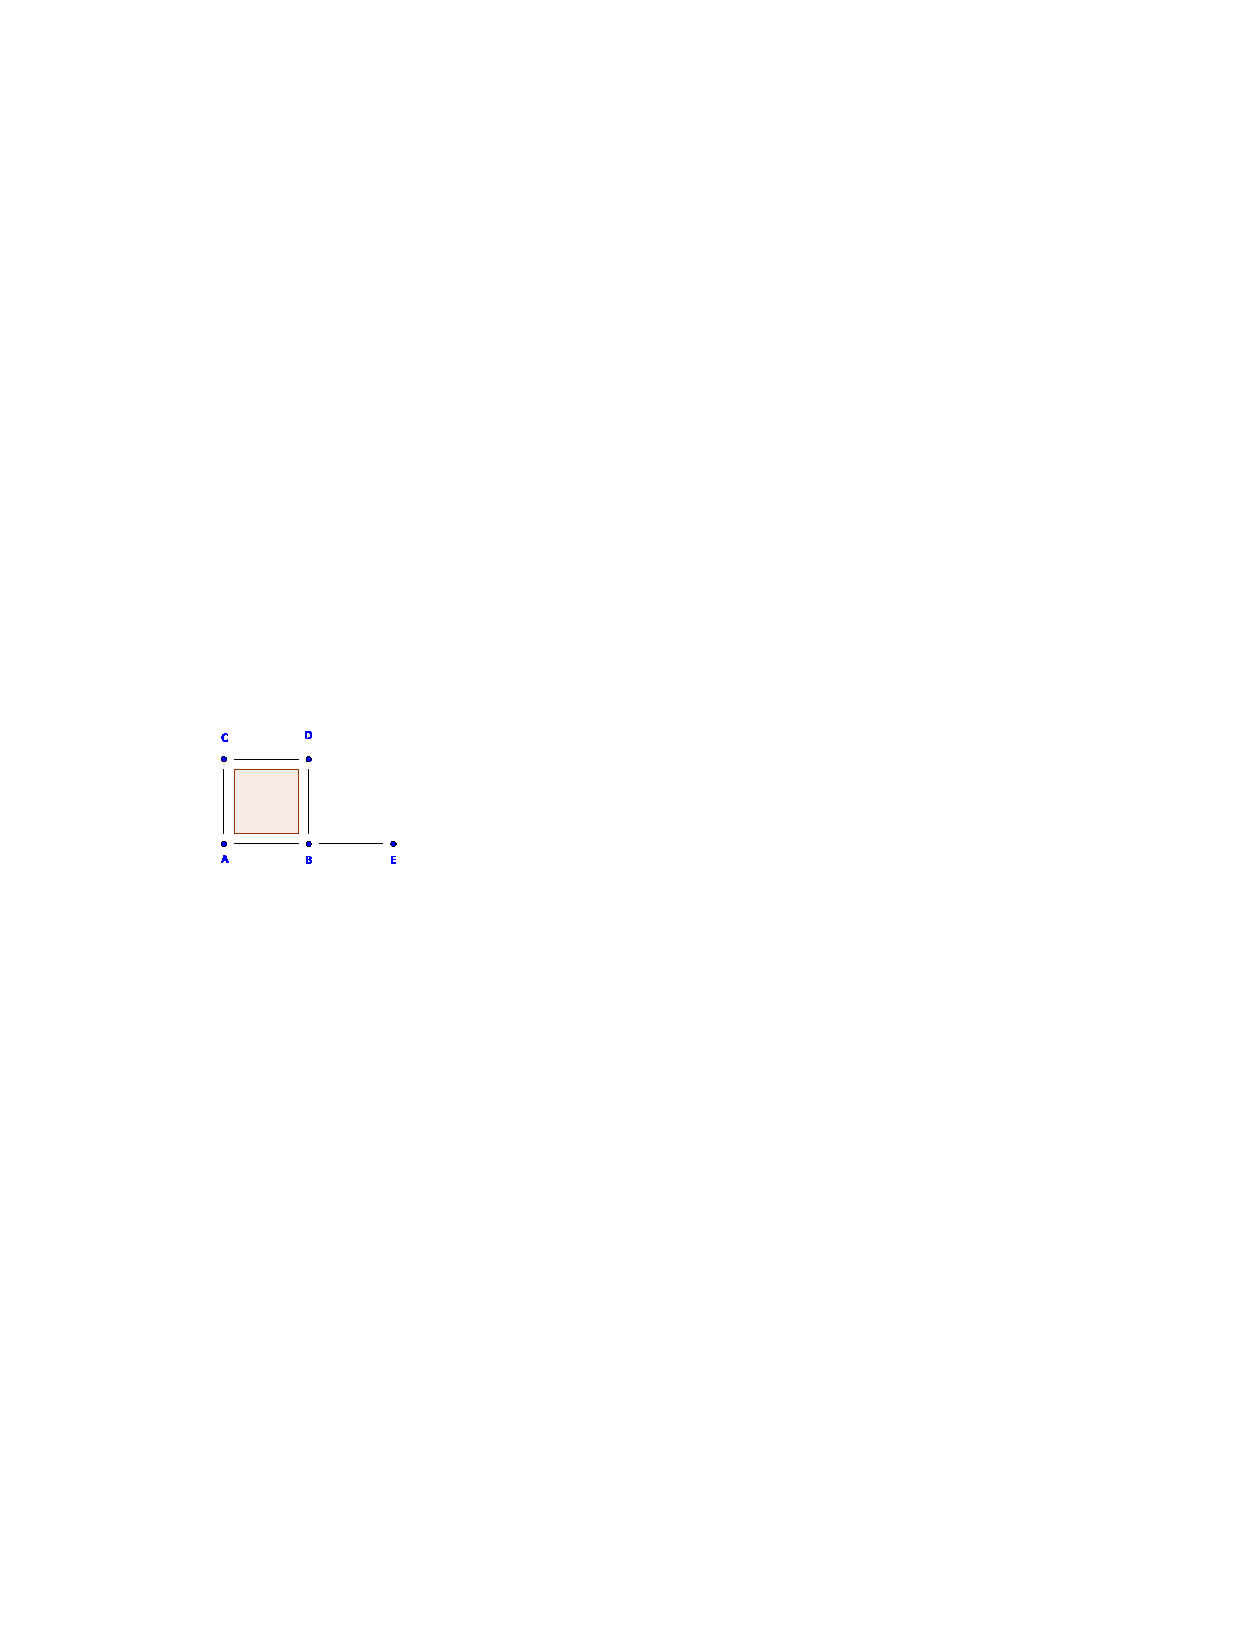
\includegraphics[trim=37mm 130mm 140mm 120mm, clip]{EjemploColapso0.pdf}}
 \subfigure[]{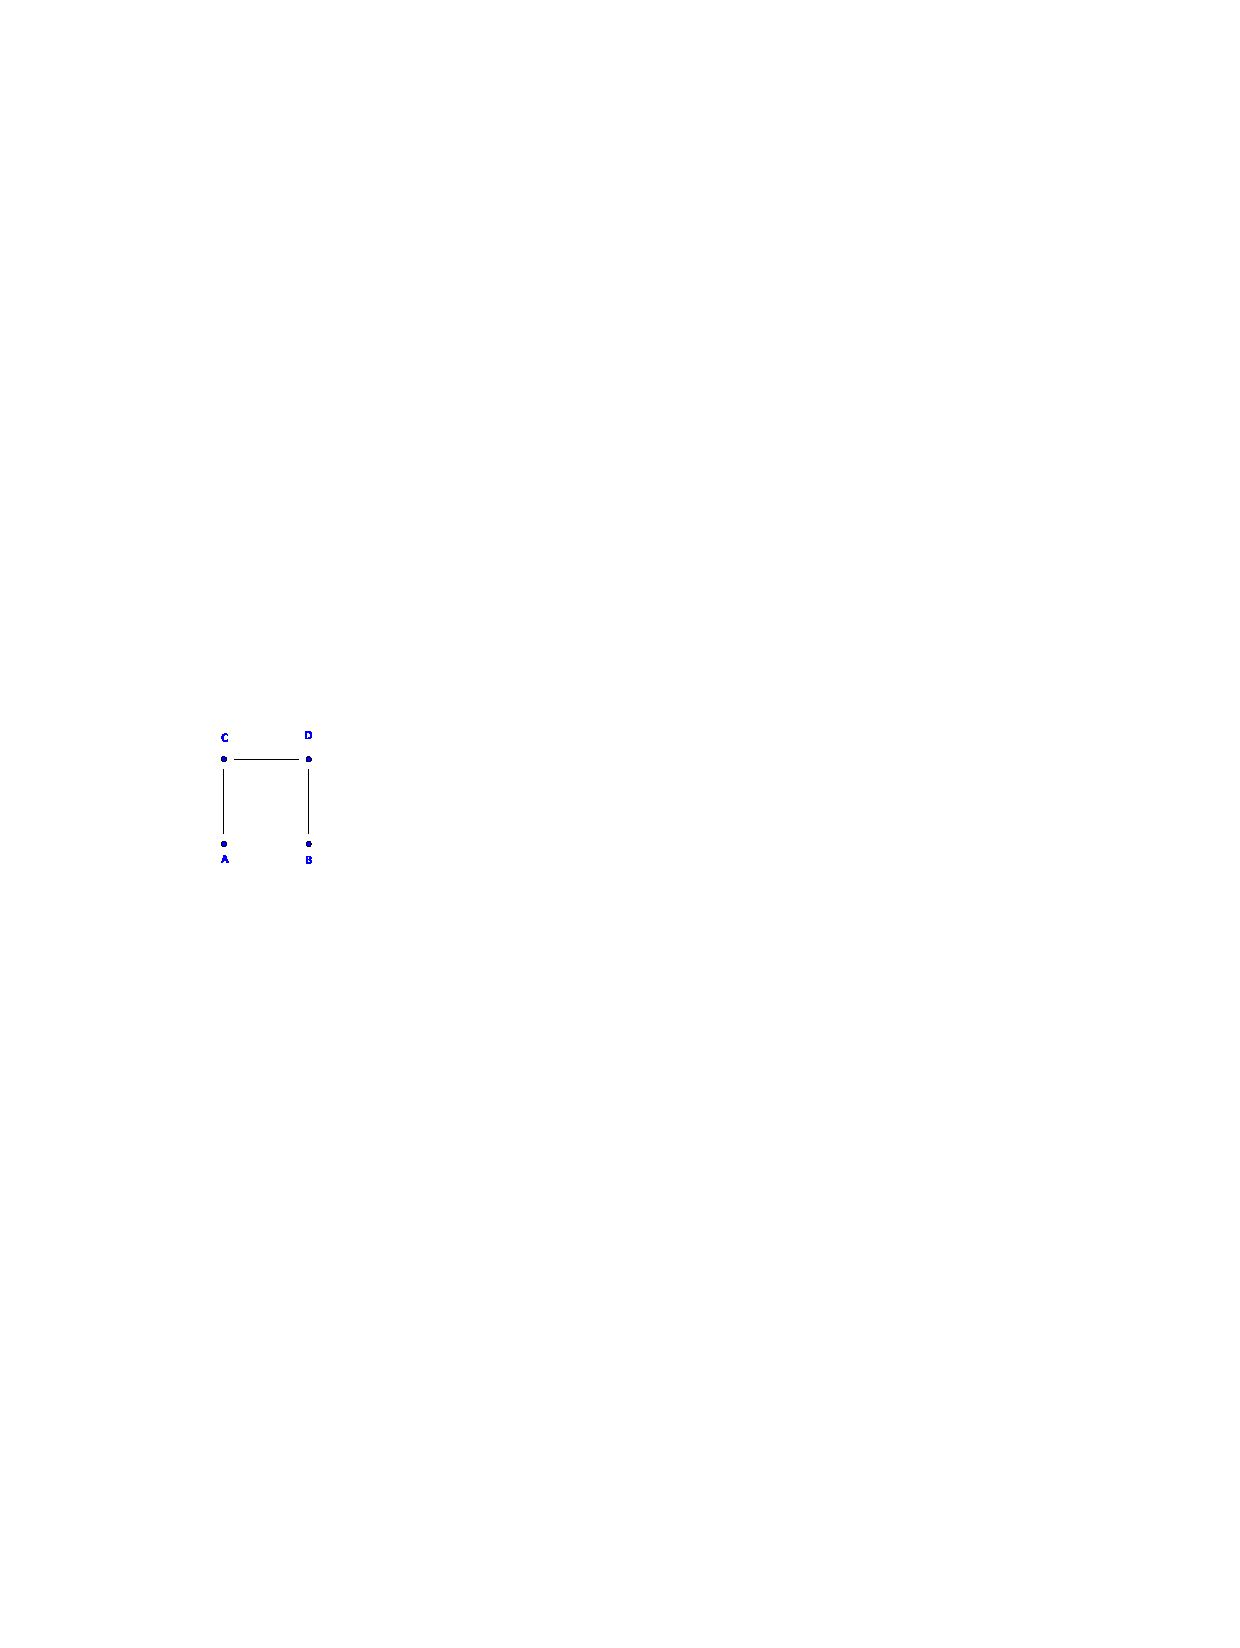
\includegraphics[trim=37mm 130mm 140mm 120mm, clip]{EjemploColapso1.pdf}}
\end{center}
 \caption{\label{Fig1} (a) Example of cubical complex. (b) Elementary collapse example: $E$ collapses onto $BE$ and
 $AC$ collapses onto $ABDC$ in the image at the left, producing the image at the
 right.}
\end{figure}

Figure \ref{Fig1} (left) shows the cubical complex
$$K=\{ABCD,AC,CD,BD,AB,BE,A,B,C,D,E\}$$ This cubical complex has 1 cell of
dimension 2 $(ABCD)$, 5 cells of dimension 1 $(AC,CD,BD,AB,BE)$ and 5 cells of
dimension 0 $(A,B,C,D,E)$. The cells $ABCD$ and $BE$ are isolated. The cells
$AC$, $CD$, $BD$ $AB$ and $E$ are free faces, but $A$, $B$, $C$ and $D$ are not
free faces, since they are proper faces of more than 1 cell complex.
The cell
$E$ is a free face of $BE$ and, hence, we can consider the elementary collapse
of $BE$ by E. The effect of such elementary collapse is the removal of $E$ and
$BE$ from the cell complex $K$. Analogously, $AC$ is a free face of $ABCD$. The
elementary collapse of $ABCD$ by $AC$ is the removal of both cells ($ABCD$ and
$AC$) from $K$. Figure \ref{Fig1} (right) shows the final cubical complex
obtained after both collapses.

\section{Liu's Algorithm} \label{sec:Liu}
As shown in the introduction, finding a skeleton for a given $d$-D image is an 
useful tool in various areas. In this paper we will introduce a bioisnpired 
parallel solution to the problem of finding a skeleton for a given $d$-D image, 
denoted as $d-\mathbf{ThCub}$.

In Liu's work \cite{liu20093d}, a cell complex is processed in order to obtain
another complex with the same topology, and the same geometry. The input cell
complex is processed by consecutive parallel removal of certain cells. The
removal process is a simple homotopy equivalence and the set of non-removed cells will make the skeleton. In Algorithm \ref{alg:CellSkel}, we present a sketch of the process of thinning implemented by Liu \emph{et al.} in \cite{liu20093d}. We use $\pi_2$ for the second coordinate projection, defined as $\pi_2(\langle \delta, \sigma \rangle) = \sigma$ for the pair $\langle \delta, \sigma \rangle$.
\begin{algorithm}[t]
 \caption{Cell complex thinning algorithm} \label{alg: Cell thinning}
 \label{alg:CellSkel}
 \begin{algorithmic}
 \REQUIRE $K$ cell complex, $\varepsilon_a, \varepsilon_r > 0$
 \FORALL{$\sigma \in K$ isolated}
 \STATE $I(\sigma) \leftarrow 0$
 \ENDFOR
 \STATE $\mbox{iter} \leftarrow 1$
 \REPEAT
 \STATE Let $S = \{\langle \delta, \sigma \rangle: \langle \delta, \sigma
 \rangle \mbox{ is a simple pair}\}$
 \STATE Let $S' =\{\langle \delta, \sigma \rangle \in S:I(\sigma)=0 \vee
 \MP_{abs}(\sigma) < \varepsilon_a \vee \MP_{rel}(\sigma) < \varepsilon_r\}$
 \STATE Let $S''$ be the greatest subset of $S'$ such that $$\forall \langle \delta_1, \sigma_1 \rangle, \langle \delta_2, \sigma_2 \rangle \in S'', \delta_1 = \delta_2 \rightarrow \sigma_1 = \sigma_2$$
 \FORALL{$\sigma \in \pi_2(S)$}
 \STATE $R(\sigma) \leftarrow \mbox{iter}$
 \ENDFOR
 \STATE $K \leftarrow K \setminus \{\sigma, \delta: \langle \delta, \sigma \rangle \in S''\}$
 \FORALL{$\sigma \in K$ new isolated cell}
 \STATE $I(\sigma) \leftarrow \mbox{iter}$
 \ENDFOR
 \STATE $\mbox{iter} \leftarrow \mbox{iter} + 1$
 \UNTIL{$S' = \emptyset$}
 \end{algorithmic}
\end{algorithm}

Let $K$ be a cubical cell complex and let $\partial$ be its border
operator. As previously seen, if only simple pairs of cells are removed, the
topology is kept. Nonetheless, in order to keep the {\it information} of the
image, some geometrical features must be preserved. For such a geometry
preservation it is necessary to require some additional properties to those
cells to be removed.

The basic idea of the algorithm is to define an iterative process where {\it
outer} cells are removed. Here, the idea of {\it outer} cells makes reference to
simple pairs, since in a simple pair $\langle \delta, \sigma \rangle$ the cell
$\delta$ is a {\it terminal} cell as it does not lie in the border of any other
one rather than $\sigma$.

In the process of iterative thinning, given a cell $\sigma$, we will denote the
later iteration when $\sigma$ is the facet of a simple pair by $R(\sigma)$. The
earlier iteration when $\sigma$ becomes isolated will be denoted by $I(\sigma)$.
Liu \emph{et al.} describe in \cite{DBLP:journals/cgf/LiuCLJ10} the relation
between $I(\sigma)$ and $R(\sigma)$, and the maximum \emph{isotropic} elongation
in $p+1$ and $p$ directions, respectively, since $\dim \sigma = p$. Thus, if
$\sigma$ is a $p$-cell in a cell complex, $I(\sigma)$ measures the shortest
discrete distance from $\sigma$ to the object boundary. This distance gives an
idea of the size of the maximum disk centered at $\sigma$ and inscribed in the
object. On the other hand, $R(\sigma)$ measures the longest distance from
$\sigma$ to the object boundary going along the skeleton $(p-1)$-cells.

From the observation of the behaviour of previous measures, Liu {\it el al.}
defined two \emph{difference measures}. The absolute one, $R(\sigma)-I(\sigma)$,
is called \emph{absolute medial persistence} and is denoted by $\MP_{abs}$. On
the other hand, \emph{relative medial persistence} is defined as
$1-\frac{I(\sigma)}{R(\sigma)}$ and denoted by $\MP_{rel}$. Both of them measure
the duration in which a cell remains isolated during thinning process.

The cell complex thinning algorithm is shown in Algorithm \ref{alg: Cell
thinning}. It starts by initializing the isolated cells. Next, the thinning
iterations start. In each iteration, all simple pairs are selected, all the
pairs where the facet cell has one of the medial persistence measures less than
given thresholds or are initially isolated are chosen, taking into account that, if 
$\langle \delta, \sigma_1\rangle$ and $\langle \delta, \sigma_2 \rangle$ are simple 
pairs that can be removed, only one of them is selected to be deleted from the complex, 
non-deterministically chosen. Finally, the cells in
selected simple pairs are removed from the cell complex.

If no cell has been removed, the thinning iterations stop,
otherwise, the iteration counter increases and the thinning
iterations continue. When the algorithm halts, a cell complex
representing the skeleton for the initial one is obtained.

\section{Membrane Computing Algorithm}\label{sec:MCA}
In previous sections two key concepts have been reviewed. On one side, cell
complexes provide an useful link between continuous spaces and discrete
structures where combinatorial algorithms may be developed using
well-established properties and results by continuous topology. On the other
hand, it has been settled a theoretical framework for working with images,
considering them as a function from a topological discrete space to a set of
{\it features}.

Our main goal is, starting from a $d$-dimensional binary image, to build other
image which represents a skeleton for the original one. In this process, a cell
complex from the original image is obtained, it is skeletonized and a new image
from the last skeleton is obtained. Of course, no topological or shape
information must be lost. The set of points\footnote{The reader is supposed to
be familiar with concepts of Image Algebra. For a detailed text, see
\cite{DBLP:journals/cvgip/RitterWD90}.} for our source images
will be the set $T_n^d = \{0,1,\ldots, n-1\}^d \subset \mathbb{Z}^d$ equipped
with a \emph{cubic} neighbourhood function, described as follows: Two points
$\mathbf{i}=(i_1, \ldots, i_p, \ldots, i_d)$ and $\mathbf{j}=(j_1, \ldots, j_p,
\ldots, j_d)$ are to be said $(2d)$-adjacent if $i_l=j_l$ for $l \neq p$ and $|i_p
- j_p| = 1$, for some $p \in \{1, 2, \ldots, d\}$. More formally, the 
neighbourhood function is given by
$$
N(i_1,\ldots, i_d) = \left\{(j_1,\ldots, j_d) \in T_n^d: \sum_{p=1}^d |j_p-i_p| = 1 \right\}
$$ 
This neighborhood function, when restricted to $d=2$, gives the 4-adjacency,
and 6-adjacency when $d=3$.

Let $I:T_n^d \rightarrow \{0,1\}$ be a $d$-D binary image of size $n^d$, where
the set of points in the object (or black points) is $I^{-1}(1)$. Let $K = K(I)$
be the cubic cell complex built from $I$. In $K$, the 0-cells represent points
in the object, the 1-cells represent pairs of $(2d)$-adjacent points, the 2-cells
represent unit squares where its edges are pairs of $(2d)$-adjacent points, and so
on. In general, each $p$-cell is a $p$-dimensional unit hypercube whose edges
are pairs of $(2d)$-adjacent points.

As we have shown in section \ref{sec:CC}, a (cubical) cell $\sigma$ is a product of intervals
$I_1 \times I_2 \times \ldots \times I_d$. We will encode $\sigma$ as the tuple 
$$
\mathbf{i} = (\inf I_1 + \sup I_1, \ldots, \inf I_k + \sup I_d)
$$

Let us denote $\mathcal{K}^d(n)$ the set of cubic cells such that the extremes of its 
elementary intervals are integers in $\{0, 1, \ldots, n-1\}$.
\begin{lemma}
The function $\mathbb{T}:\mathcal{K}^d(n) \rightarrow T_{2n-1}^d$ defined by
$$
\mathbb{T}(I_1 \times I_2 \times \cdots \times I_d) = 
(\inf I_1 + \sup I_1, \ldots, \inf I_d + \sup I_d)
$$ is a bijection.
\end{lemma}
\begin{proof}
First of all, $\mathbb{T}$ is well defined as, for all $\sigma = I_1 \times \cdots \times I_d$ is 
$0 \leq \inf I_p, \sup I_p \leq n-1$ for each $p \in \{1, \ldots, d\}$, therefore 
$0 \leq \inf I_p + \sup I_p \leq 2(n-1)$ and $\mathbb{T}(\sigma) \in T_{2n-1}^d$.

Let us prove that $\mathbb{T}$ is injective. Let $\sigma_1, \sigma_2 \in \mathcal{K}^d(n)$ 
be two different cells. Let us denote $I_p(\sigma)$ as the $p$-th elementary interval 
in $\sigma$. As $\sigma_1 \neq \sigma_2$, let us suppose that $I_p(\sigma_1) \neq I_p(\sigma_2)$ 
for some $p \in \{1, \ldots, d\}$. If both elementary intervals are degenerated, as they are different, 
both $\sup I_p(\sigma_1)$ and $\sup I_p(\sigma_2)$ are different too, so 
$\mathbb{T}(\sigma_1) \neq \mathbb{T}(\sigma_2)$. If both intervals are non-degenerated, 
as they are different and its extremes are pairs of consecutive integers, 
$\sup I_p(\sigma_1) \neq \sup I_p(\sigma_2)$ and $\mathbb{T}(\sigma_1) \neq \mathbb{T}(\sigma_2)$. 
If one elementary interval is degenerated and the other is non-degenerated, 
$\mathbb{T}(\sigma_1) \neq \mathbb{T}(\sigma_2)$ as the $p$-th coordinate of one of them is even as the 
corresponding coordinate of the other is odd. Note that $\sup (l, l+1) + \inf (l, l+1) = 2l+1$ while 
$\sup [l] + \inf [l] = 2l$. Therefore, $\mathbb{T}$ is a bijection.

To prove that $\mathbb{T}$ is surjective, it is enough to find a cell $\sigma \in \mathcal{K}^d(n)$ for
a given tuple $(l_1, \ldots, l_d) \in T_{2n-1}^d$. Let us denote $\mathbf{I}(s)$ as follows
$$
\mathbf{I}(s)= \left \{ 
\begin{array}{ll}
\left(\frac{s-1}{2}, \frac{s+1}{2}\right)		& \textbf{if } s \equiv 1 (\mod 2)\\
\left[\frac{s}{2}\right]						& \textbf{if } s \equiv 0 (\mod 2)
\end{array}
\right.
$$
Let us define $\sigma = \mathbf{I}(l_1) \times \cdots \times \mathbf{I}(l_d)$. As $0 \leq l_p \leq 2n-2$ for 
each $p \in \{1, \ldots, d\}$, $\sigma \in \mathcal{K}^d(n)$. If $l_p$ is odd, 
$\sup \mathbf{I}(l_p) + \inf \mathbf{I}(l_p) = l_p$ and, if $l_p$ is even then 
$\sup \mathbf{I}(l_p) + \inf \mathbf{I}(l_p) = l_p$ too. Hence, $\mathbb{T}(\sigma) = (l_1, \ldots, l_d)$.
\end{proof}

Note that, as the dimension of a cell is the number of non-degenerated intervals in its definition, 
the dimension of a cell given as a tuple is the amount of odd coordinates.

As an example, the cell $\sigma=(0,1) \times [2] \times (5,6)$ in $\mathbf{R}^3$ is encoded as
$\mathbb{T}(\sigma) = (0+1, 2+2, 5+6)= (1, 4, 11)$.

As we have defined above, the border operator $\partial: \mathcal{K}^d \rightarrow 2^{\mathcal{K}^d}$ 
returns the set $\partial\, \sigma$ of principal faces for any cell $\sigma$. More over, it is easy to prove
that $\partial (\mathcal{K}^d(n)) \subset 2^{\mathcal{K}^d(n)}$. Hence the following commutative diagram
gives us an appropiate definition of border operator for cubical cells represented as tuples:
$$
\begin{CD}
\mathcal{K}^d (n) 	@>\mathbb{T}>> 	T_{2n-1}^d \\
@VV{\partial}V						@VV{\partial}V\\
2^{\mathcal{K}^d(n)} @>2^\mathbb{T}>> 2^{T_{2n-1}^d}
\end{CD}
$$
where $2^\mathbb{T}(K)=\{\mathbb{T}(\sigma): \sigma \in K\}$

The operator $\partial: T_{2n-1}^d \rightarrow 2^{T_{2n-1}^d}$ can be defined, hence, as follows:
$$
\partial \mathbf{i} = 2^\mathbb{T} \circ \partial \circ \mathbb{T}^{-1} (\mathbf{i})
$$
where its explicit expression is given by
\begin{eqnarray*}
\partial \mathbf{i} = 
\{\mathbf{d}^-_p(\mathbf{i}):1 \leq p \leq d \wedge i_p \equiv 1 (\mod 2)\} \cup\\ 
\{\mathbf{d}^+_p(\mathbf{i}):1 \leq p \leq d \wedge i_p \equiv 1 (\mod 2)\}
\end{eqnarray*}
where $\mathbf{i} = (i_1, \ldots, i_d)$; $\mathbf{d}^-_p$ and $\mathbf{d}^+_p$ are defined as follows
$$
\mathbf{d}^-_p(i_1, \ldots, i_p, \ldots, i_d) = (i_1, \ldots, i_p-1, \ldots, i_d)
$$
$$
\mathbf{d}^+_p(i_1, \ldots, i_p, \ldots, i_d) = (i_1, \ldots, i_p+1, \ldots, i_d)
$$
Therefore, as an example, 
$$
\partial (1,4,11) = \{(0,4,11), (1,4,10)\} \cup \{(2,4,11), (1,4,12)\}
$$

Next, we provide the description of the P systems used as a Membrane
Computing implementation of the Algorithm \ref{alg:CellSkel}, all of them 
consisting on five membranes. The first membrane is used as input and for 
marking the isolated cells before starting the thinning iterations. The second 
membrane is used to mark simple pairs. The third membrane selects the cells
to be removed, removes the marked cells and updates the facet
counter. The fourth membrane marks new isolated cells, updates
counters $I$ and $R$. The fifth one is used as output membrane.
Next, our tissue P system is formally described.

In order to properly denote the number of facets of a cell we will use
the \emph{star} operator, defined as follows:
$$
\mathrm{st}\,\sigma= \{\mu \in K: \sigma \in \partial \mu\}
$$
for any cell $\sigma$ in a cell complex $K$. Making a little abuse of notation, 
we will also represent as $\mathrm{st}$ to the operator 
$$
2^\mathbb{T} \circ \mathrm{st} \circ \mathbb{T}^{-1} : T_{2n-1}^d \rightarrow 2^{T_{2n-1}^d}
$$
determined in the following commutative diagram:
$$
\begin{CD}
\mathcal{K}^d (n) 	@>\mathbb{T}>> 	T_{2n-1}^d \\
@VV{\mathrm{st}}V						@VV{\mathrm{st}}V\\
2^{\mathcal{K}^d(n)} @>2^\mathbb{T}>> 2^{T_{2n-1}^d}
\end{CD}
$$

Recall that, given a finite set $A$, $\#A$ denotes the number of elements in $A$.

In the following paragraphs we will define a family of tissue P systems to solve the 
$d-\mathbf{ThCub}$ problem. This P systems find an skeleton for a cubical complex $K$
while the topology (in terms of homotopy equivalence) and shape is kept. The P systems
are designed to work following the next sequence of steps:
\begin{list}{Step \arabic{enumi}:}{\usecounter{enumi}}
\item Mark initially isolated cells in the input membrane.
\item Move objects from the first membrane to second one.
\item Mark simple pairs. \label{itm:SimplePairs}
\item Move objects from the second membrane to the third.
\item Mark cells to be removed.
\item Remove marked cells and update some counters.
\item Move objects from the third membrane to the fourth.
\item If no cell has been removed in previous steps, send skeleton cells to the output 
membrane and halts. In other case, move objects from fourth membrane to fifth.
\item Update counters.
\item Move objects from the fifth membrane to the second and continue from Step \ref{itm:SimplePairs}.
\end{list}
Let $I$ be a $d$-D binary image of size $n^d$, let $K$ be the cubical cell complex built
from $I$, let $\varepsilon_{abs} \in \{1, 2, \ldots, n\}$ and $\varepsilon_{rel}
\in \{\tau_1, \ldots, \tau_m\} \subset (0,1) \cap \mathbb{Q}$, where $\tau_j <
\tau_{j+1}$ for $1 \leq j < m$. For every tuple $\langle n, \varepsilon_{abs},
\varepsilon_{rel} \rangle$ we will define a tissue P system with promoters,
inhibitors, priorities and input, denoted by $\Pi(n, \varepsilon_{abs},
\varepsilon_{rel})$ and defined as follows:
$$
 \Pi(n, \varepsilon_{abs}, \varepsilon_{rel}) =
 (\Gamma,\Sigma,\mathcal{E},w_1,\dots,w_6,\mathcal{R},Pri,i_{in},i_o)
$$
where:
\begin{itemize}
    \item $\Gamma = \{\mathbf{i}: \mathbf{i} \in T_{2n-1}^d\} \cup \{(R,
    \mathbf{i}, z), (I, \mathbf{i}, z): \mathbf{i} \in T_{2n-1}^d, 1 \leq z \leq
    2n\}\cup$ \newline $\cup\{F_\mathbf{i}:\mathbf{i} \in
    T_{2n-1}^d\}\cup\{I_\mathbf{i}, \overline{I}_\mathbf{i}, S_\mathbf{i},
    \overline{S}_\mathbf{i}, R_\mathbf{i}, \overline{R}_\mathbf{i}, U_\mathbf{i}:
    \mathbf{i} \in T_{2n-1}^d\} \cup \{R, H\}$
    \item $\Sigma =
    \{\mathbf{i},(R,\mathbf{i},1),(I,\mathbf{i},0),F_\mathbf{i}^{\#\mathrm{st}\,\mathbf{i}}:
    \mathbf{i} \in K\}$
    \item $w_1 = \ldots = w_6 = \emptyset$
    \item $\mathcal{E} = \Gamma \setminus \Sigma$
\end{itemize}

 The rules in the P system will be determined by the use of rule
schemes. A rule scheme is a set of rules where some elements inside
them are given as parameters in some set. From this point of view, a
rule scheme is a function from some set of parameters to the set of
rules of the system.

$\mathcal{R}$ is the set of rules:
\begin{itemize}
%% R1
    \item
    $\Rule{}{}{F_\mathbf{i},I_\mathbf{i}}{1}{\mathbf{i}}{\mathbf{i}\,I_\mathbf{i}}{0}{\mathbf{i}
    \in T_{2n-1}^d}$.
%% R2
    \item
    $\Rule{}{F_\mathbf{i}^l}{F_\mathbf{i}^{l+1},\overline{I}_\mathbf{i}}{1}{\mathbf{i}}{\mathbf{i}\,\overline{I}_\mathbf{i}}{0}{\mathbf{i}
    \in T_{2n-1}^d, 1 \leq l \leq 2d}$

    These rules mark every isolated cell $\mathbf{i}$ with \emph{isolation mark}
    $I_\mathbf{i}$ and every non isolated cell $\mathbf{i}$ with \emph{non
    isolation mark} $\overline{I}_\mathbf{i}$.
%% R3
    \item $\Rule{}{}{}{1}{F_\mathbf{i}}{}{2}{\mathbf{i} \in T_{2n-1}^d}$
%% R4
    \item
    $\Rule{}{}{}{1}{\mathbf{i}\,(R,\mathbf{i},1)\,(I,\mathbf{i},0)\,I_\mathbf{i}}{}{2}{\mathbf{i}
    \in T_{2n-1}^d}$
%% R5
    \item
    $\Rule{}{}{}{1}{\mathbf{i}\,(R,\mathbf{i},1)\,(I,\mathbf{i},0)\,\overline{I}_\mathbf{i}}{}{2}{\mathbf{i}
    \in T_{2n-1}^d}$

    These rules move cells, \emph{remove counters}, \emph{isolation counters},
    \emph{facet counters} and isolation marks to the second membrane, in order to
    detect simple pairs.
%% R6
    \item $\Rule{}{}{F_\mathbf{j}^2, S_\mathbf{i},
    S_\mathbf{j}}{2}{\mathbf{i}\,\mathbf{j}\,F_\mathbf{j}}
    {\mathbf{i}\,\mathbf{j}\,F_\mathbf{j}\,S_\mathbf{i}\,S_\mathbf{j}}{0}{\mathbf{i}
    \in T_{2n-1}^d, \mathbf{j} \in \partial\,\mathbf{i}}$

    These rules detect simple pairs $\langle \mathbf{j},\mathbf{i} \rangle$ and
    mark its elements using \emph{simple pair mark} $S_\mathbf{i}$ and
    $S_\mathbf{j}$.
%% R7
    \item
    $\Rule{}{}{\overline{S}_\mathbf{i}}{2}{\mathbf{i}}{\mathbf{i}\,\overline{S}_i}{0}{\mathbf{i}
    \in T_{2n-1}^d}$.

	These rules mark every cell $\mathbf{i}$ that not belongs to any simple pair
	with the \emph{non simple pair mark} $\overline{S}_\mathbf{i}$.
%% R8
    \item $\Rule{}{\mathbf{i}}{}{2}{F_\mathbf{i}}{}{3}{\mathbf{i} \in T_{2n-1}^k}$
%% R9
    \item $\Rule{}{}{}{2}{\mathbf{i}\,(R,\mathbf{i},z)\,(I,\mathbf{i},
    Z)\,\overline{I}_\mathbf{i}\,S_\mathbf{i}}{}{3}{\mathbf{i} \in T_{2n-1}^d, 0
    \leq z, Z, \leq 2n}$
%% R10
    \item $\Rule{}{}{}{2}{\mathbf{i}\,(R,\mathbf{i},z)\,(I,\mathbf{i},
    Z)\,I_\mathbf{i}\,\overline{S}_\mathbf{i}}{}{3}{\mathbf{i} \in T_{2n-1}^d, 0
    \leq z, Z, \leq 2n}$
%% R11
    \item $\Rule{}{}{}{2}{\mathbf{i}\,(R,\mathbf{i},z)\,(I,\mathbf{i},
    Z)\,\overline{I}_\mathbf{i}\,\overline{S}_\mathbf{i}}{}{3}{\mathbf{i} \in
    T_{2n-1}^d, 0 \leq z, Z, \leq 2n}$
%% R12
    \item $\Rule{}{}{}{2}{\mathbf{i}\,(R,\mathbf{i},z)\,(I,\mathbf{i},
    Z)\,I_\mathbf{i}\,S_\mathbf{i}}{}{3}{\mathbf{i} \in T_{2n-1}^d, 0 \leq z, Z,
    \leq 2n}$

    These rules send cells, counters and markers to the third membrane, where
    cells with not enough shape information will be removed.
%% R13
    \item
    $\Rule{}{I_\mathbf{i},(I,\mathbf{i},0),S_\mathbf{i},S_\mathbf{j}}{R_\mathbf{i},
    R_\mathbf{j}}{3}{\mathbf{i}\,\mathbf{j}}{\mathbf{i}\,\mathbf{j}\,R_\mathbf{i}\,R_\mathbf{j}\,R\,H}{0}{\mathbf{i}\in
    T_{2n-1}^d, \mathbf{j} \in \partial\, \mathbf{i}}$.

	These rules mark every simple pair $\langle \mathbf{j}, \mathbf{i} \rangle$ as
	removable where the facet cell $\mathbf{i}$ is initially isolated.
%% R14
    \item $\Rule{}{S_\mathbf{i},S_\mathbf{j},(R,\mathbf{i},z),
    (I,\mathbf{i},Z)}{R_\mathbf{i},
    R_\mathbf{j}}{3}{\mathbf{i}\,\mathbf{j}}{\mathbf{i}\,\mathbf{j}\,R_\mathbf{i}\,R_\mathbf{j}\,R\,H}{0}{\mathbf{i}\in
    T_{2n-1}^d, \mathbf{j} \in \partial\, \mathbf{i}, \MP_{abs} <
    \varepsilon_{abs} \mbox{or }\MP_{rel} < \varepsilon_{rel} \mbox{ and } 0 \leq
    z,Z \leq 2n, \mbox{ where }\\\MP_{abs}=z-Z \mbox{ and
    }\MP_{rel}=1-\frac{Z}{z}}$.

	These rules mark those cells $\mathbf{i}$ and $\mathbf{j}$ such that $\langle
	\mathbf{j}, \mathbf{i} \rangle$ is a simple pair, none of them has been marked
	to be removed and the cell $\mathbf{i}$ has not enough shape meaning,
	measured in terms of medial persistence, absolute or relative.
%% R15
    \item
    $\Rule{}{}{\overline{R}_\mathbf{i}}{3}{\mathbf{i}}{\mathbf{i}\,\overline{R}_\mathbf{i}}{0}{\mathbf{i}
    \in T_{2n-1}^d}$.

    These rules mark any cell $\mathbf{i}$ as non removable, with \emph{non
    removable mark} $\overline{R}_\mathbf{i}$, if it has not been previously
    marked as removable.

%% R16
    \item $\Rule{}{\mathbf{i}, \mathbf{j}, R_\mathbf{i},
    \overline{R}_\mathbf{j}}{}{3}{F_\mathbf{j}}{}{0}{\mathbf{i} \in T_{2n-1}^d,
    \mathbf{j} \in \partial\, \mathbf{i}}$

    These rules update facet counters.
%% R17
    \item
    $\Rule{}{}{}{3}{\mathbf{i}\,(R,\mathbf{i},z)\,(I,\mathbf{i},Z)\,R_\mathbf{i}\,R\,I_\mathbf{i}}{}{0}{\mathbf{i}
    \in T_{2n-1}^d, 0 \leq z, Z \leq 2n}$
%% R18
    \item
    $\Rule{}{}{}{3}{\mathbf{i}\,(R,\mathbf{i},z)\,(I,\mathbf{i},Z)\,R_\mathbf{i}\,R\,\overline{I}_\mathbf{i}}{}{0}{\mathbf{i}
    \in T_{2n-1}^d, 0 \leq z, Z \leq 2n}$
%% R19
    \item $\Rule{}{R_\mathbf{i}}{}{3}{S_\mathbf{i}}{}{0}{\mathbf{i} \in T_{2n-1}^d}$
%% R20
    \item $\Rule{}{R_\mathbf{i}}{}{3}{\overline{S}_\mathbf{i}}{}{0}{\mathbf{i} \in T_{2n-1}^d}$
%% R21
    \item $\Rule{}{R_\mathbf{i}}{}{3}{F_\mathbf{i}}{}{0}{\mathbf{i} \in T_{2n-1}^d}$

    These rules remove those cells marked for removal.
%% R22
    \item $\Rule{}{H,\overline{R}_\mathbf{i}}{R}{3}{\mathbf{i}\,(R,\mathbf{i},z)\,(I,\mathbf{i},Z)\,I_\mathbf{i}}{}{4}{\mathbf{i} \in T_{2n-1}^d, 0 \leq z,Z \leq 2n}$
%% R23
    \item $\Rule{}{H,\overline{R}_\mathbf{i}}{R}{3}{\mathbf{i}\,(R,\mathbf{i},z)\,(I,\mathbf{i},Z)\,\overline{I}_\mathbf{i}}{}{4}{\mathbf{i} \in T_{2n-1}^d, 0 \leq z,Z \leq 2n}$
%% R24
    \item $\Rule{}{H,\overline{R}_\mathbf{i}}{R}{3}{F_\mathbf{i}}{}{4}{\mathbf{i} \in T_{2n-1}^d}$
%% R25
    \item $\Rule{}{H,\overline{R}_\mathbf{i}}{R}{3}{S_\mathbf{i}}{}{4}{\mathbf{i}\mathbf{j} \in T_{2n-1}^d}$
%% R26
    \item $\Rule{}{H,\overline{R}_\mathbf{i}}{R}{3}{\overline{S}_\mathbf{i}}{}{4}{\mathbf{i} \in T_{2n-1}^d}$
%% R27
\item $\Rule{}{}{R}{3}{H}{}{4}{}$

    These rules move remaining objects to the fourth membrane.
%% R28
    \item $\Rule{}{\overline{R}_\mathbf{i}}{H,R}{3}{\mathbf{i}}{}{5}{\mathbf{i} \in T_{2n-1}^d}$

	These rules send output to the fifth membrane.
%% R29
    \item $\Rule{}{}{\mathbf{i}, R}{3}{R_\mathbf{i}}{}{0}{\mathbf{i} \in T_{2n-1}^d}$
%% R30
    \item $\Rule{}{}{\mathbf{i}, R}{3}{\overline{R}_\mathbf{i}}{}{0}{\mathbf{i} \in T_{2n-1}^d}$
%% R31
    \item $\Rule{}{}{}{4}{S_\mathbf{i}}{}{0}{\mathbf{i} \in T_{2n-1}^d}$
%% R32
    \item $\Rule{}{}{}{4}{\overline{S}_\mathbf{i}}{}{0}{\mathbf{i} \in T_{2n-1}^d}$
%% R33
    \item $\Rule{}{}{}{4}{H}{}{0}{}$

    These rules remove auxiliary objects for each removed cell.
%% R34
\item $\Rule{}{(R,\mathbf{i},z)}{F_\mathbf{i}}{4}{\mathbf{i}\,\overline{I}_\mathbf{i}\,(I,\mathbf{i},Z)}{\mathbf{i}\,I_\mathbf{i}\,(I,\mathbf{i},z)}{0}{\mathbf{i} \in T_{2n-1}^d, 0 \leq z,Z \leq 2n}$
%% R35
    \item $\Rule{}{F_\mathbf{i}}{U_\mathbf{i}}{4}{\mathbf{i}}{\mathbf{i}}{0}{\mathbf{i} \in T_{2n-1}^d}$

    These rules update isolation counter and isolation marks.
%% R36
    \item $\Rule{}{}{U_\mathbf{i}}{4}{\mathbf{i}\,(R,\mathbf{i},z)}{\mathbf{i}\,(R,\mathbf{i}, z+1)\,U_\mathbf{i}}{0}{\mathbf{i} \in T_{2n-1}^d, 1 \leq z \leq 2n-1}$

    These rules update removal counter.
%% R37
    \item $\Rule{}{U_\mathbf{i}}{}{4}{\mathbf{i}\,(R,\mathbf{i},z)\,(I,\mathbf{i},Z)\,I_\mathbf{i}}{}{2}{\mathbf{i} \in T_{2n-1}^d, 0\leq z,Z \leq 2n}$
%% R38
    \item $\Rule{}{U_\mathbf{i}}{}{4}{\mathbf{i}\,(R,\mathbf{i},z)\,(I,\mathbf{i},Z)\,\overline{I}_\mathbf{i}}{}{2}{\mathbf{i} \in T_{2n-1}^d, 0\leq z,Z \leq 2n}$
%% R39
    \item $\Rule{}{U_\mathbf{i}}{}{4}{F_\mathbf{i}}{}{2}{\mathbf{i} \in T_{2n-1}^d}$

    These rules move objects to the second membrane.
\end{itemize}
Finally, we complete the description of the tissue P systems with $Pri$, $i_{in}$ and $i_{out}$.

\begin{itemize}
    \item $Pri = \{R_6 > R_7, R_{13} > R_{15}, R_{14} > R_{15}, R_{36} > R_{34}\} $
    \item $i_{in} = 1$ is the input cell.
    \item $i_{out} = 5$ is the output cell.
\end{itemize}

\begin{theorem}
The family of P Systems $\Pi(n, \varepsilon_{abs}, \varepsilon_{rel})$ defined above builds an skeleton for the
cubical complex built from a $d$-D image, $d=2,3$, in logarithmic time (measured as number of computation steps 
with respect to the size of the input image $n^d$). 
\end{theorem}
\begin{proof}

Let $K \subset T_{2n-1}^k$ be the cubical cell complex encoded as described above for a given $d$-D image.

The evolution of the P systems follows the steps sequenced below.
\begin{list}{\textbf{Step \arabic{enumi}}}{\usecounter{enumi}}
%% Paso 1
\item In this step only rules establishing communication with the first membrane
can be selected, hence only rules from $R_1$ to $R_5$ can be taken
up. However, rules $R_4$ and $R_5$ require the presence of isolation
marks, either positive ($I_\mathbf{i}$) or negative
($\overline{I}_\mathbf{i}$), and those marks are not present yet
into the first membrane. Consequently, only rules $R_1$, $R_2$ and
$R_3$ can be selected. The application of the selected rules in the
scheme $R_1$, import from the environment an isolation mark
$I_\mathbf{i}$ for each isolated cell $\mathbf{i}$. Also, the
application of rules in $R_2$ take one non isolation mark
$\overline{I}_\mathbf{i}$ for every non isolated cell $\mathbf{i}$.
The application of the rules in the scheme $R_3$ moves every facet
counter $F_\mathbf{i}$ to the second membrane.
%% Paso 2
\item In this situation, only rules in the five first schemes can be selected.
However, the presence of isolation marks blocks the selection of
rules $R_1$ and $R_2$. On the other hand, facet counters have been
moved to the second membrane in the prior step. Henceforth, only
rules $R_4$ and $R_5$ can be selected.

After the application of the selected rules, all the available objects are in
the second membrane.
%% Paso 3
\item In this computation stage, with all the objects inside the second
membrane, only rules in the schemes $R_6$ to $R_{12}$ can be selected. Rules in
$R_9$ through $R_{12}$ cannot be selected as there is no simple pair marks,
either positive or negative. Rules $R_6$, $R_7$ and $R_8$ determine a maximal
set of rules bearing in mind that rules in $R_6$ has greater priority than rules
in $R_7$ and both of them take all the available cells objects $\mathbf{i}$.

After applying the selected rules, every cell in the second membrane has a
simple pair mark, either positive or negative. In addition, the application of
rules in $R_8$ moves the facet counters to the third membrane.
%% Paso 4
\item Only rules in the schemes $R_6$ to $R_{12}$ can
be selected, as any other one has not enough elements in the corresponding
membrane to be chosen. On the other hand, in the present stage the presence of
simple pair marks prevent the selection of rules $R_6$ or $R_7$ and the absence
of facet counters $F_\mathbf{i}$ avoid the selection of rules in $R_8$. Hence,
only rules from $R_9$ to $R_{12}$ can be selected.

The application of selected rules leads the system to the following computation,
with all the objects in the third membrane.
%% Paso 5
\item In this step, only rules in $R_{13}$ through $R_{15}$ can be selected. All
of them determine a maximal set of rules that marks every cell $\mathbf{i}$ as
removable or not removable, bearing in mind the priority relation $R_{13} >
R_{14} > R_{15}$.

After the application of selected rules, all the cells are marked with remove
mark, either positive or negative. Although, for each cell marked as removable,
one object $R$ and one object $H$ have been imported from the environment.
%% Paso 6
\item In this computation stage, all the cells have been marked as removable or
not removable. Here we can find two different possibilities, depending on the
existence of objects $R_i$, $R$ and $H$, marking the remove of some cells.
\begin{list}{\arabic{enumii})}{\usecounter{enumii}}
\item If no cell has been marked as removable, there are no objects
$R_\mathbf{i}$, $R$ or $H$ in the third membrane. In this situation, rules
$R_{16}$ through $R_{27}$ cannot be selected as all of them requiere the
presence either of objects $R_\mathbf{i}$, $R$ or $H$. On the other hand, rules
in $R_{29}$ and $R_{30}$ cannot be selected as they require the absence of
objects $\mathbf{i}$. The rules from $R_{31}$ above cannot be neither selected,
as the take objects from the fourth membrane and, in the present situation,
there are no objects inside it.

The only rules that can be selected are those in the scheme $R_{28}$. After its
application, all the cells are inside the output membrane, the fifth one. This
situation prevent the selection of any rule, resulting in a halting computation.
\item Let us suppose now that there are some cells marked to be removed inside the third
membrane. Henceforth, there are objects $R_\mathbf{i}$, $R$ and $H$ for each
cell marked as removable. The only rules that can be selected are those in
$R_{16}$ through $R_{21}$. The rules in $R_{22}$ up to $R_{30}$ cannot be
selected in this stage as they require the absence of objects $R$. Rules from
$R_{31}$ above cannot be selected as they require the presence of objects
inside the fourth membrane and, in the current stage, this membrane is empty.

The application of the selected rules updates the facet counter
($R_{16}$), removes cells, simple pair marks and facet counters for
each removable cell ($R_{17}$ to $R_{21}$).
\end{list}
%% Paso 7
\item To reach this configuration it is essential to have removed some cells in
prior steps. After removing all the cells marked to be removed, all the objects
$R$ have been removed too. This allows the rules $R_{22}$ up to $R_{27}$ to be
selected. The other rules cannot be selected as they require the presence of
objects that there are not present inside the corresponding membrane.

The application of the selected rules leads the system to the next
configuration, where all the objects are inside the fourth membrane.
%% Paso 8
\item In this computation, only the rules in $R_{29}$ up to $R_{35}$ can be
selected. Rules $R_{34}$ and $R_{35}$ have been designed to make a maximal set
of rules, as every object $\mathbf{i}$ can be used by only one of them.

The application of the selected rules erases auxiliary objects ($R_{29}$ to
$R_{33}$), marks new isolated cells and update counter $I$ ($R_{34}$).
%% Paso 9
\item In this stage, the only rules that can be selected are those in $R_{36}$
due to priority reasons ($R_{36} > R_{35}$). Rules in $R_{37}$ up to $R_{39}$
require the presence of objects $U_\mathbf{i}$ and those objects are not
present yet inside the fourth membrane.

The application of the selected rules updates the counter $R$.
%% Paso 10
\item Now, only the rules $R_{37}$ up to $R_{39}$ can be
selected. After the application of the selected rules, all the available objects
are inside the second membrane, allowing the system to evolve repeating the
steps shown below.
\end{list}

\end{proof}

The required computational resources for the family of tissue P systems defined
in this paper is given in the table \ref{table: Complexity Aspects}.
\begin{table}[t!]
\begin{center}
\begin{tabular}{|c|}
\hline
$d$-D binary image thinning problem ($d-\mathbf{ThCub}$)\\
\hline
\end{tabular}\\
\begin{tabular}{|l|c|}
	\hline
	\textbf{Complexity}                     &  \\ 
	\hline
	Number of steps of computation          & $\leq 8d(n+1)+6$ \\ 
	\hline\hline
	\textbf{Resources needed}               &  \\ 
	\hline
	Size of the alphabet                    &   $O(n^{d+1})$   \\
	Initial number of cells                 &       $5$        \\
	Initial number of objects               &     $O(|K|)$     \\
	Number of rules                         &   $O(n^{d+2})$   \\
	Upper bound for the length of the rules &       $8$        \\ 
	\hline
\end{tabular}\caption{Complexity aspects, where the size of the input data is $O(n^d)$,
$|K|$ is the number of cells in the input cell complex $K$.}\label{table: Complexity Aspects}
\end{center}
\end{table}

\subsection{Example}
In order to proper understanding of the parallel bioinspired algorithm presented in this 
paper, we will show here a simple example. We will start with a binary 2-D image shown in
Figure \ref{fig:Example01}(a), where each pixel is represented as a square. In Figure 
\ref{fig:Example01}(b) the cubical complex associated to the input image is shown over the 
source image and, finally, the associated cubical complex is presented alone in Figure 
\ref{fig:Example01}(c). In all of the previous figures a coordinate system is presented. 
The last one presents the encoding used in this paper to represent a cubic cell by a tuple of 
integers. For example, the cell $(3,5)$ in Figure \ref{fig:Example01}(c) is the only square in
the complex. In the following paragraphs we show the thinning process using thresholds 
$\varepsilon_{abs}=2$ and $\varepsilon_{rel}=0.5$.
 
Figure \ref{fig:Example01}(d) presents one of the simple pairs that can be selected for removal,
e.g. $\langle (2,8), (2,7) \rangle$ and $\langle (4,5), (3,5) \rangle$. Recall that, when a cell
belongs to many simple pairs, one of them is non-deterministically chosen. The counters 
$I$ and $R$ for the facets of those simple pairs are $I(2,7)=I(3,5)=0$ as both cells are initially
isolated and $R(2,7)=R(3,5)=1$ as they are selected to be removed in the first iteration. Therefore,
the medial persistence measures are given by
\begin{eqnarray*}
\MP_{abs}(2,7)=1, \MP_{rel}(2,7)=1,\\
\MP_{abs}(3,5)=1, \MP_{rel}(3,5)=1
\end{eqnarray*}
 
Hence, both simple pairs can be removed resulting in the complex given in Figure \ref{fig:Example01}(e). 

In the next iteration, the simple pairs are shown (in red) in Figure \ref{fig:Example01}(f). 
The values for isolation and remove counter for the facet of the only one simple pair are, respectively,
$I(3,6)=1$ as it became isolated in the first iteration and $R(3,6)=2$ as it was selected for removal in
the second iteration. Medial persistence values are given by
$$
\MP_{abs}(3,6)=1, \MP_{rel}(3,6)=0.5
$$
Hence, the only simple pair can be removed, obtaining the complex in Figure \ref{fig:Example01}(g).

Once again, there is only one simple pair (shown in Figure \ref{fig:Example01}(h)) where 
isolation and removal counters values are, respectively, $I(2,5)=1, R(2,5)=3$. Therefore, 
the medial persistence measures are given by
$$
\MP_{abs}(2,5)=2, \MP_{rel}(2,5) \approx 0.67
$$
so it cannot be removed, as this simple pair retains shape information.

Finally, the algorithm halts returning the complex in Figure \ref{fig:Example01}(i).
\begin{figure}
\label{fig:Example01}
\subfigure[]{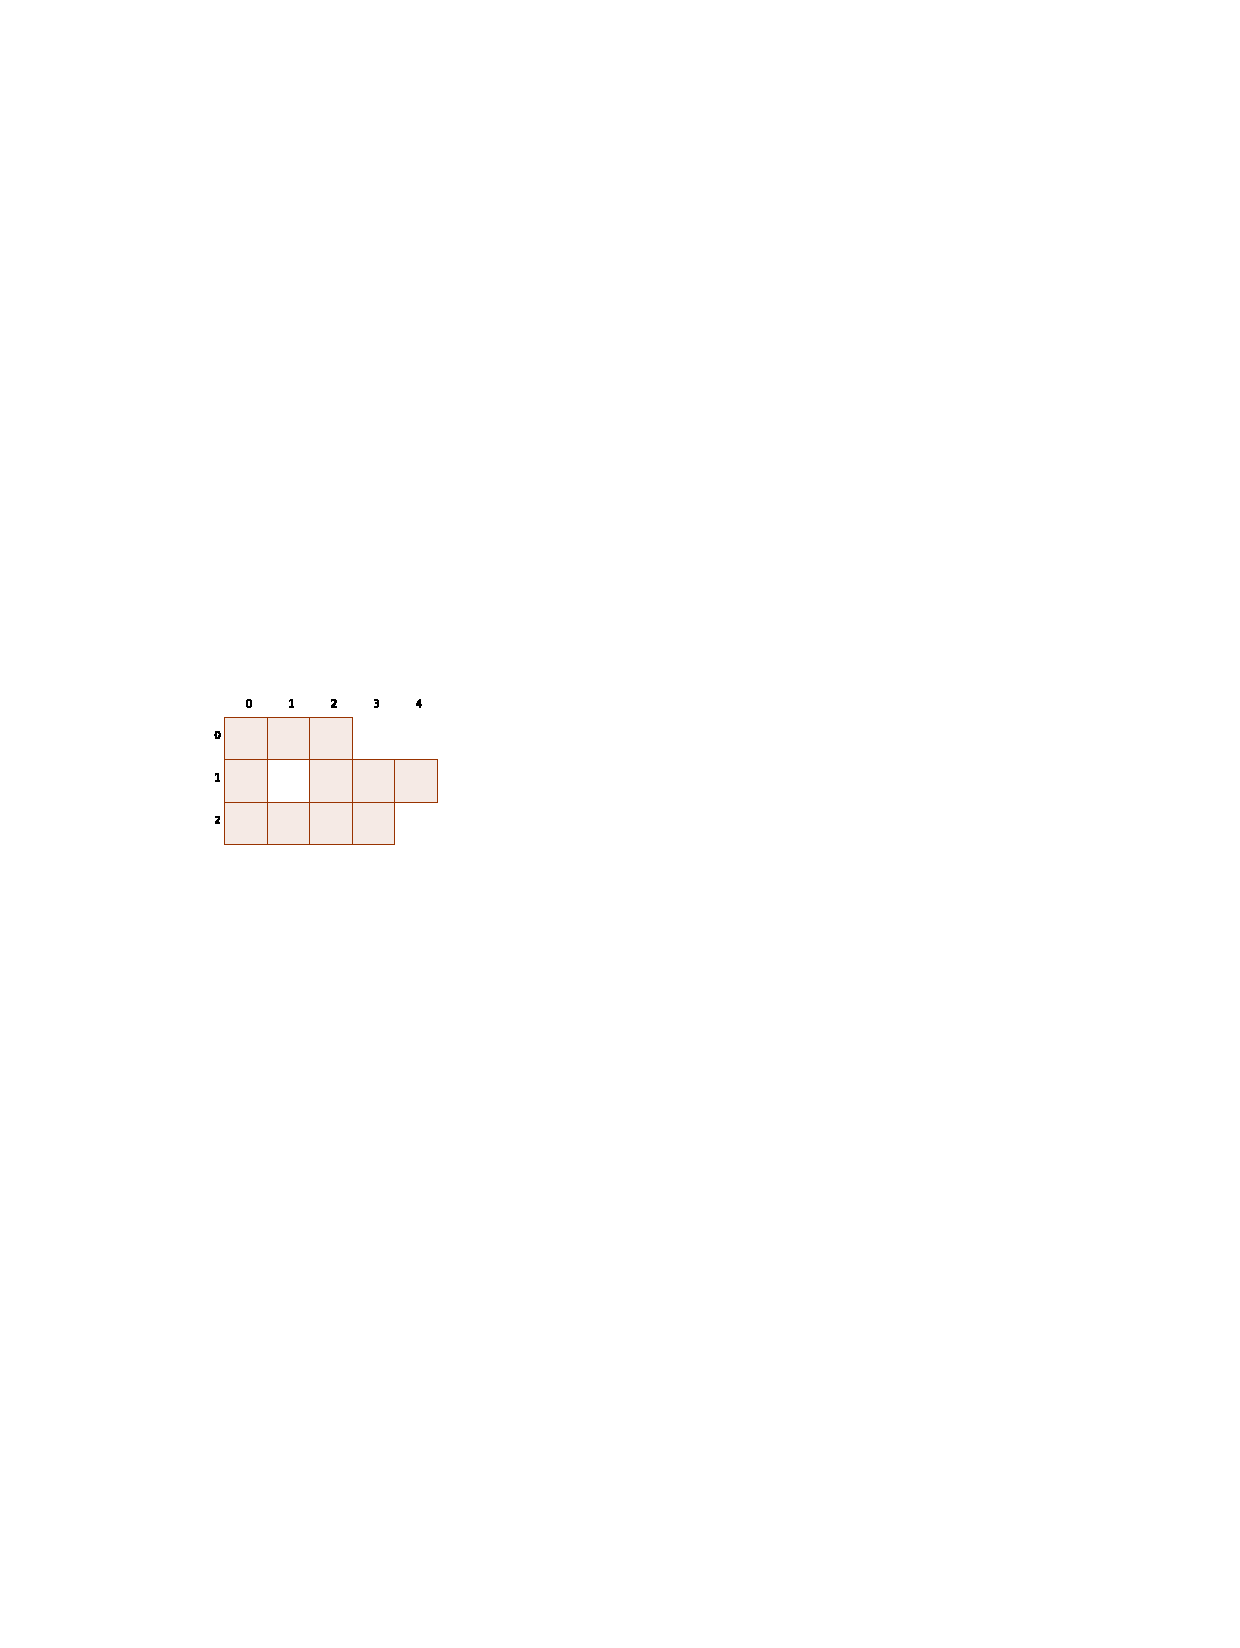
\includegraphics[trim=35mm 135mm 135mm 115mm, clip]{Example-01.pdf}}
\subfigure[]{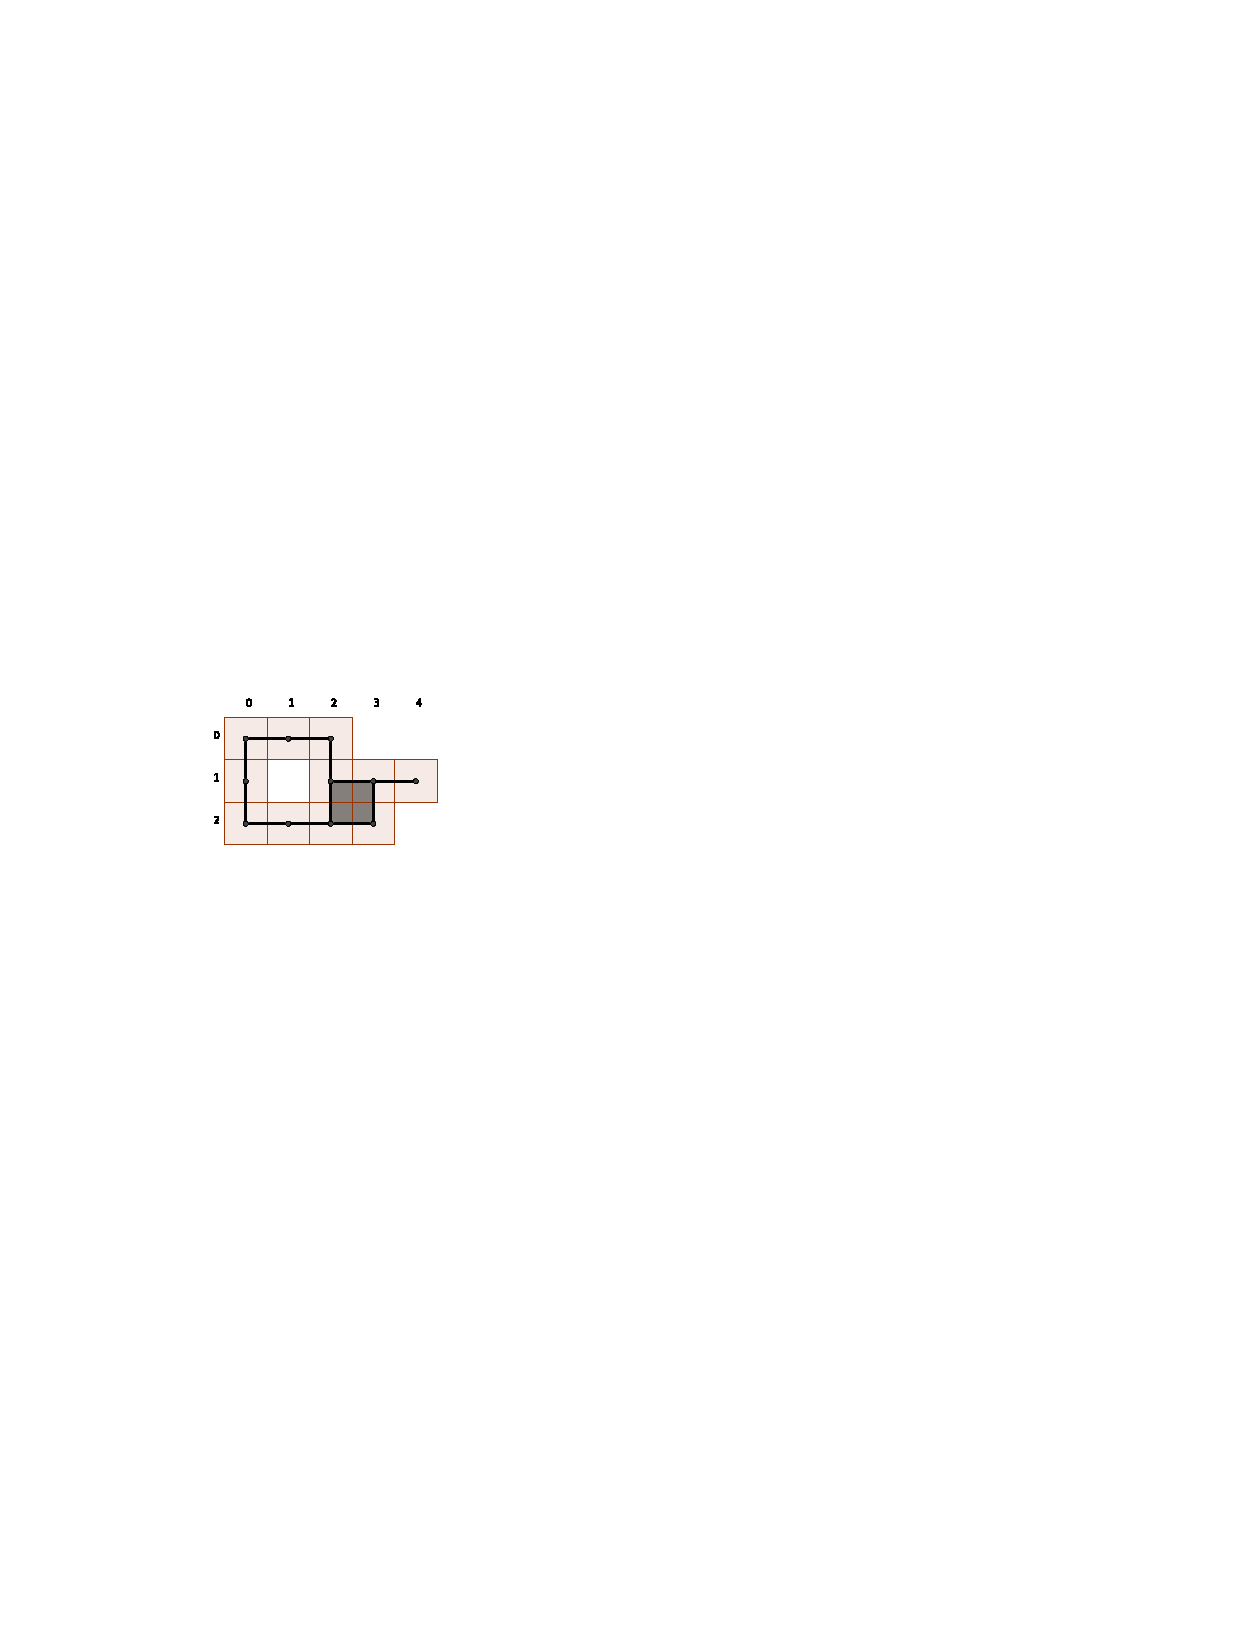
\includegraphics[trim=35mm 135mm 135mm 115mm, clip]{Example-02.pdf}}
\subfigure[]{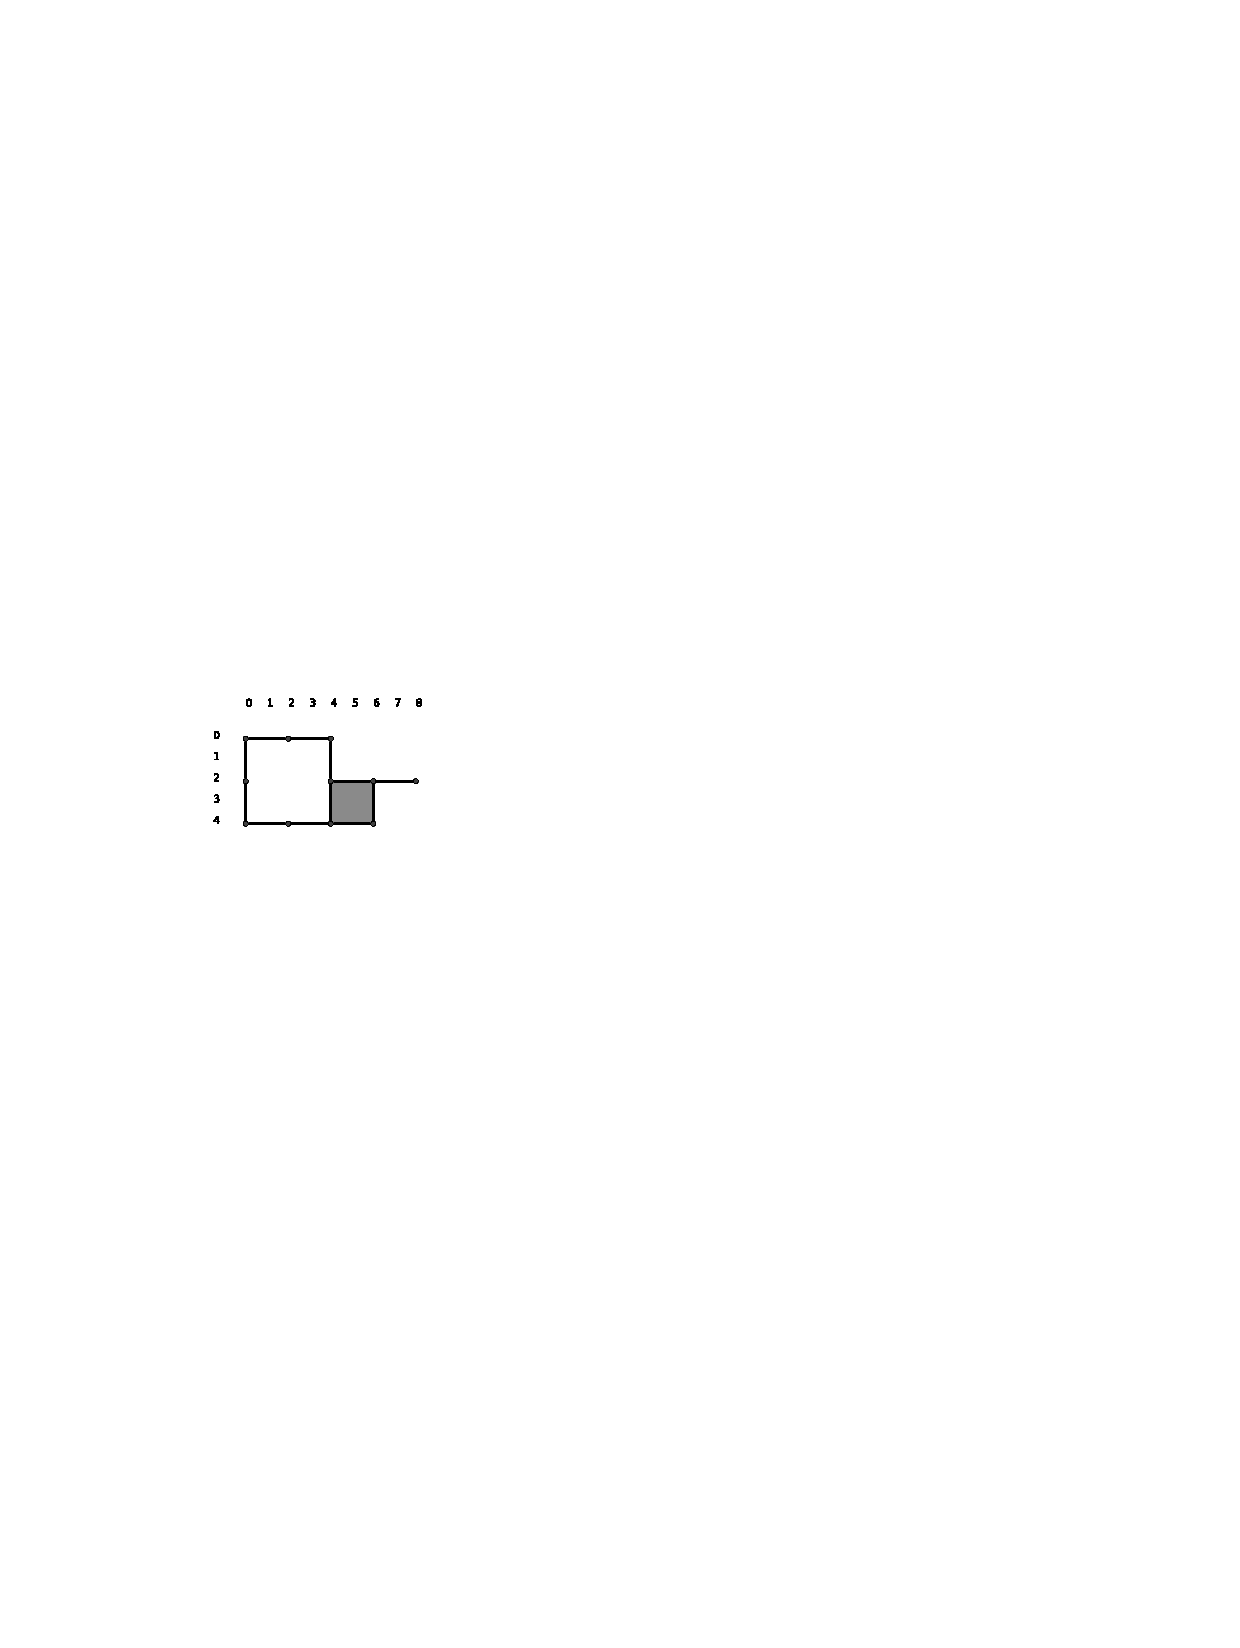
\includegraphics[trim=35mm 135mm 135mm 115mm, clip]{Example-04.pdf}}\\
\subfigure[]{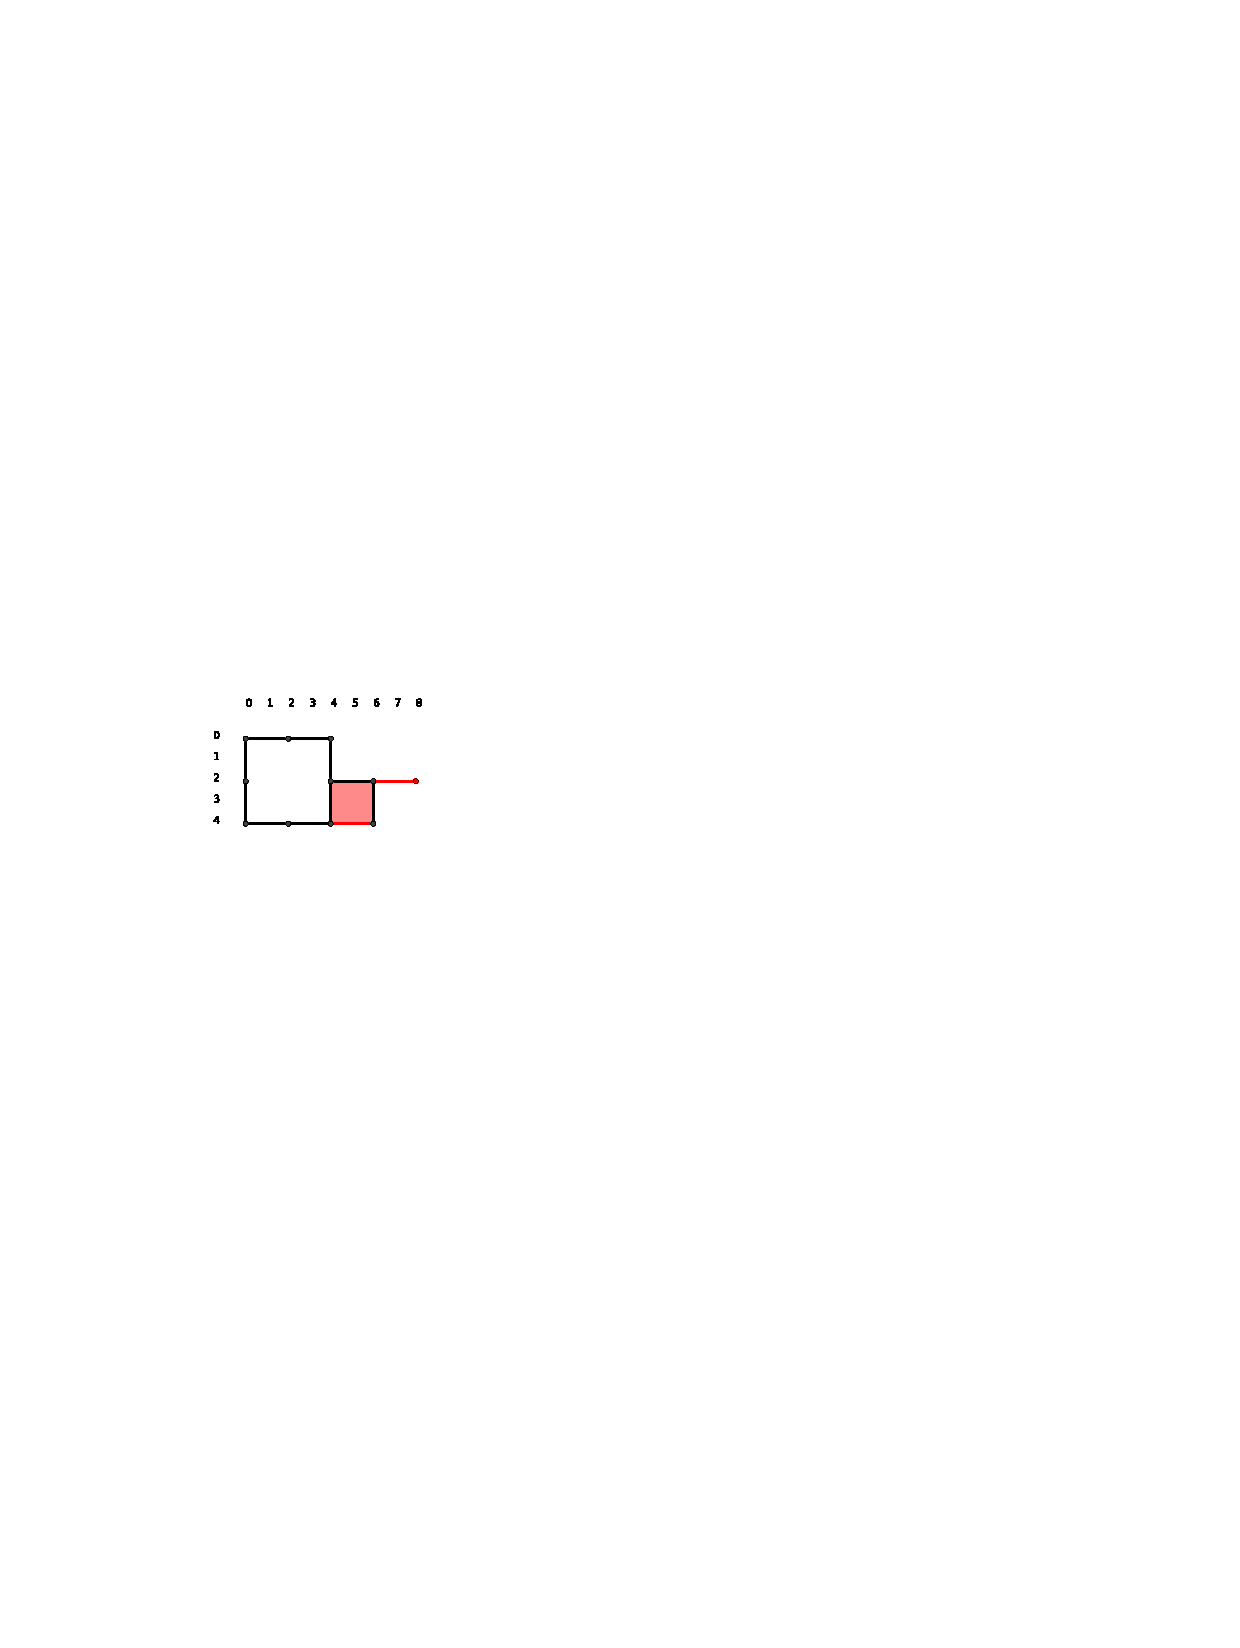
\includegraphics[trim=35mm 135mm 135mm 115mm, clip]{Example-06.pdf}}
\subfigure[]{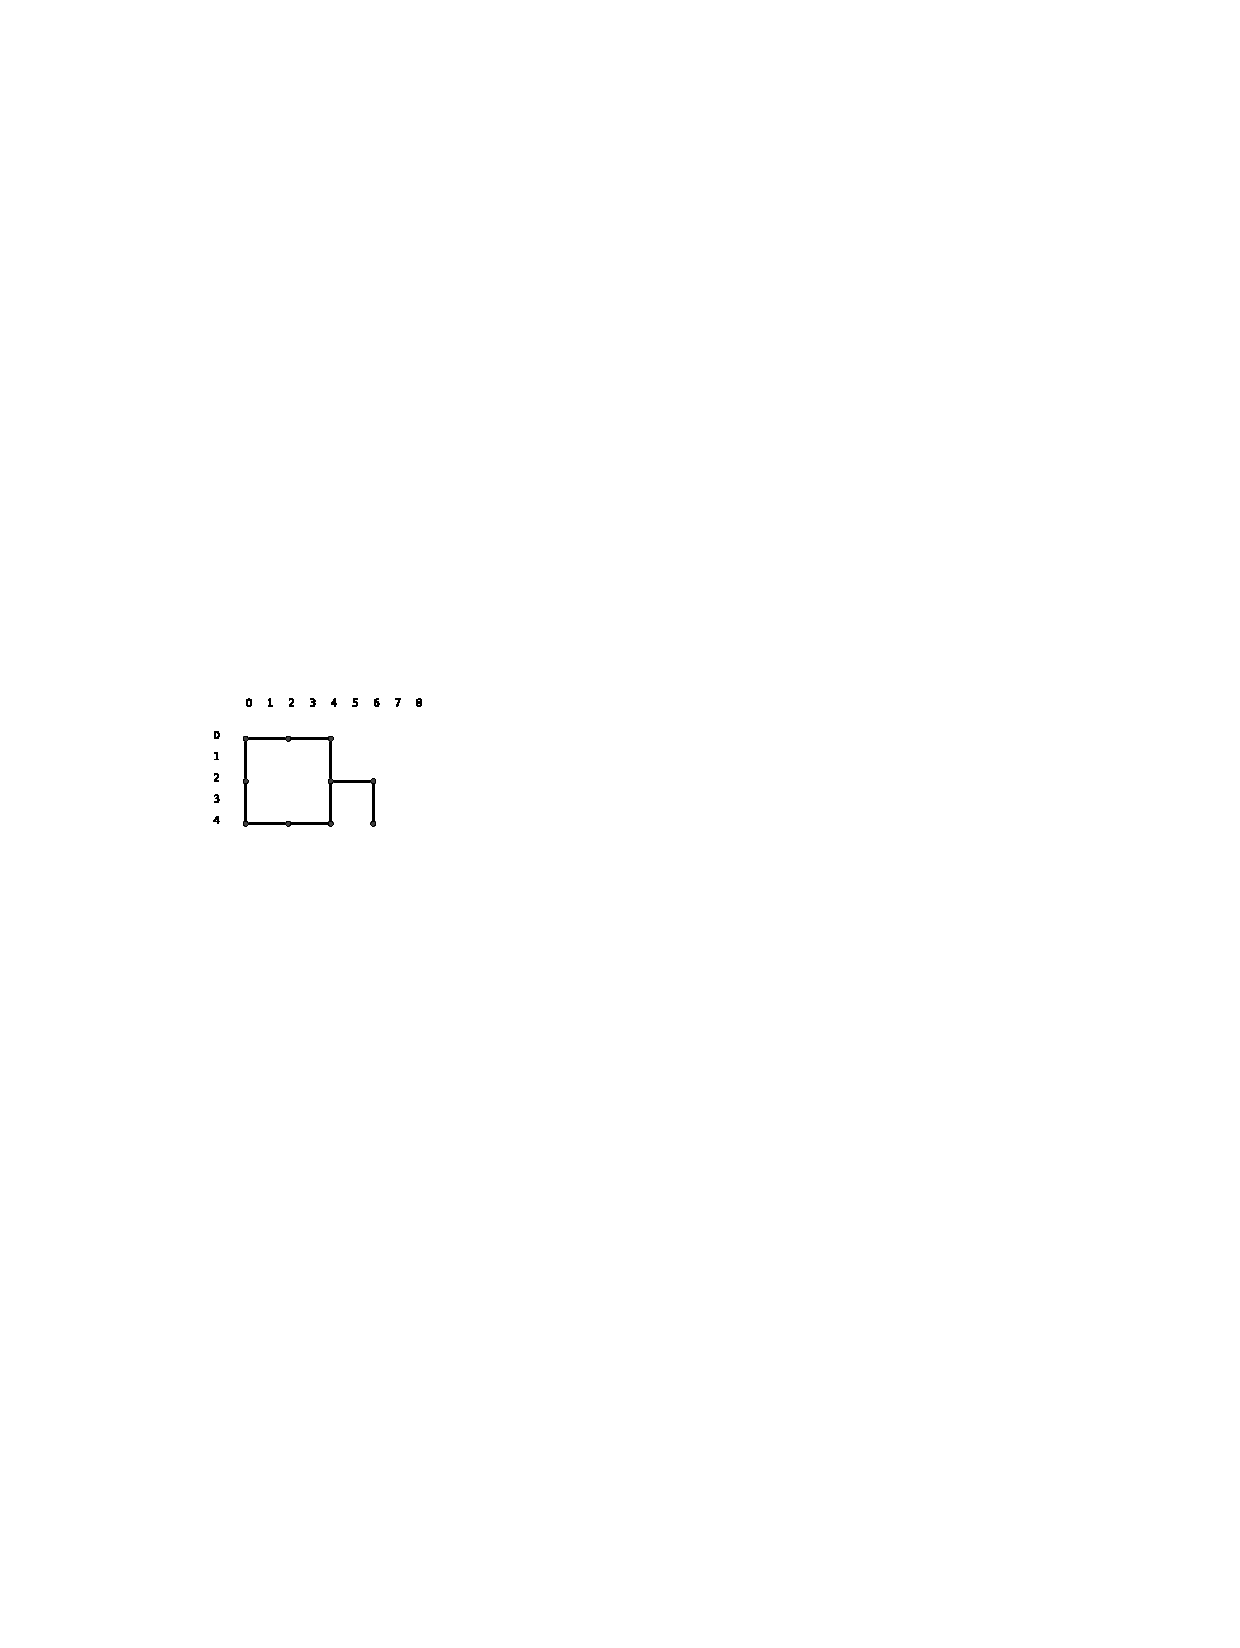
\includegraphics[trim=35mm 135mm 135mm 115mm, clip]{Example-07.pdf}}
\subfigure[]{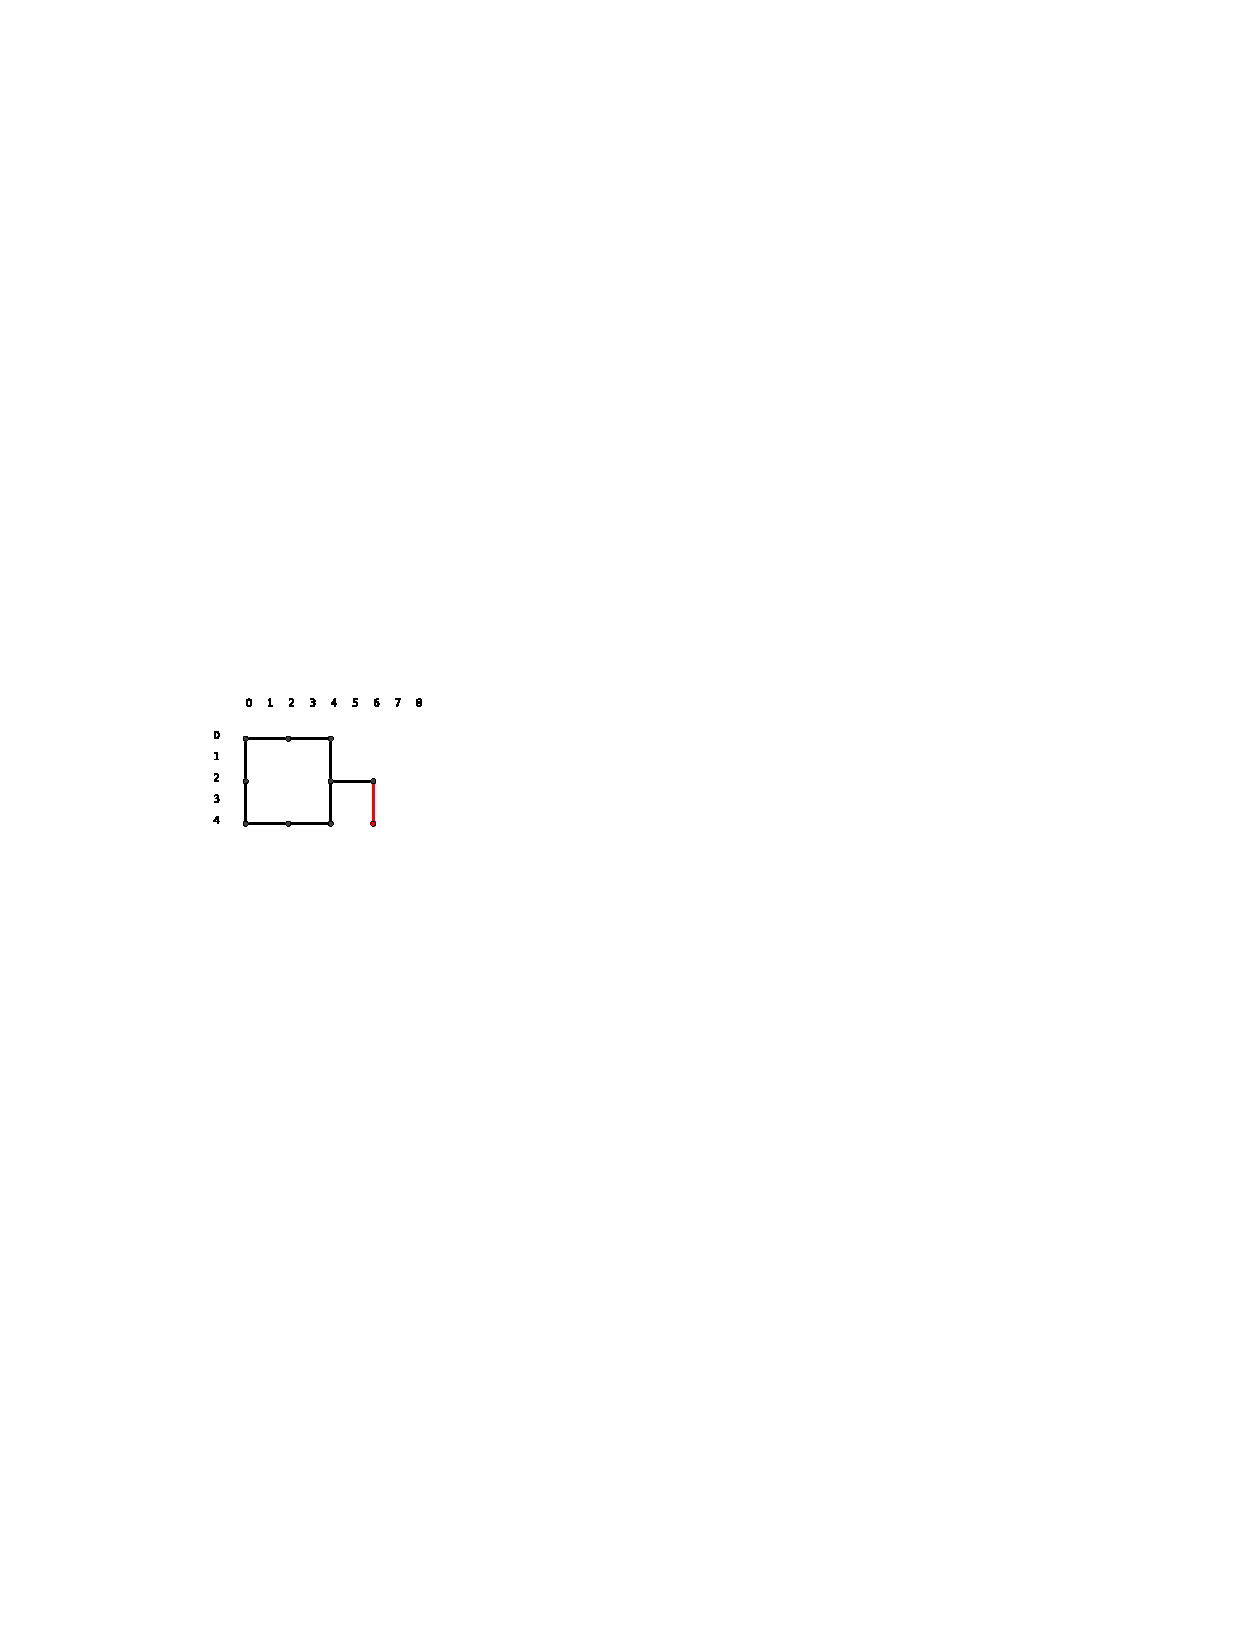
\includegraphics[trim=35mm 135mm 135mm 115mm, clip]{Example-08.pdf}}\\
\subfigure[]{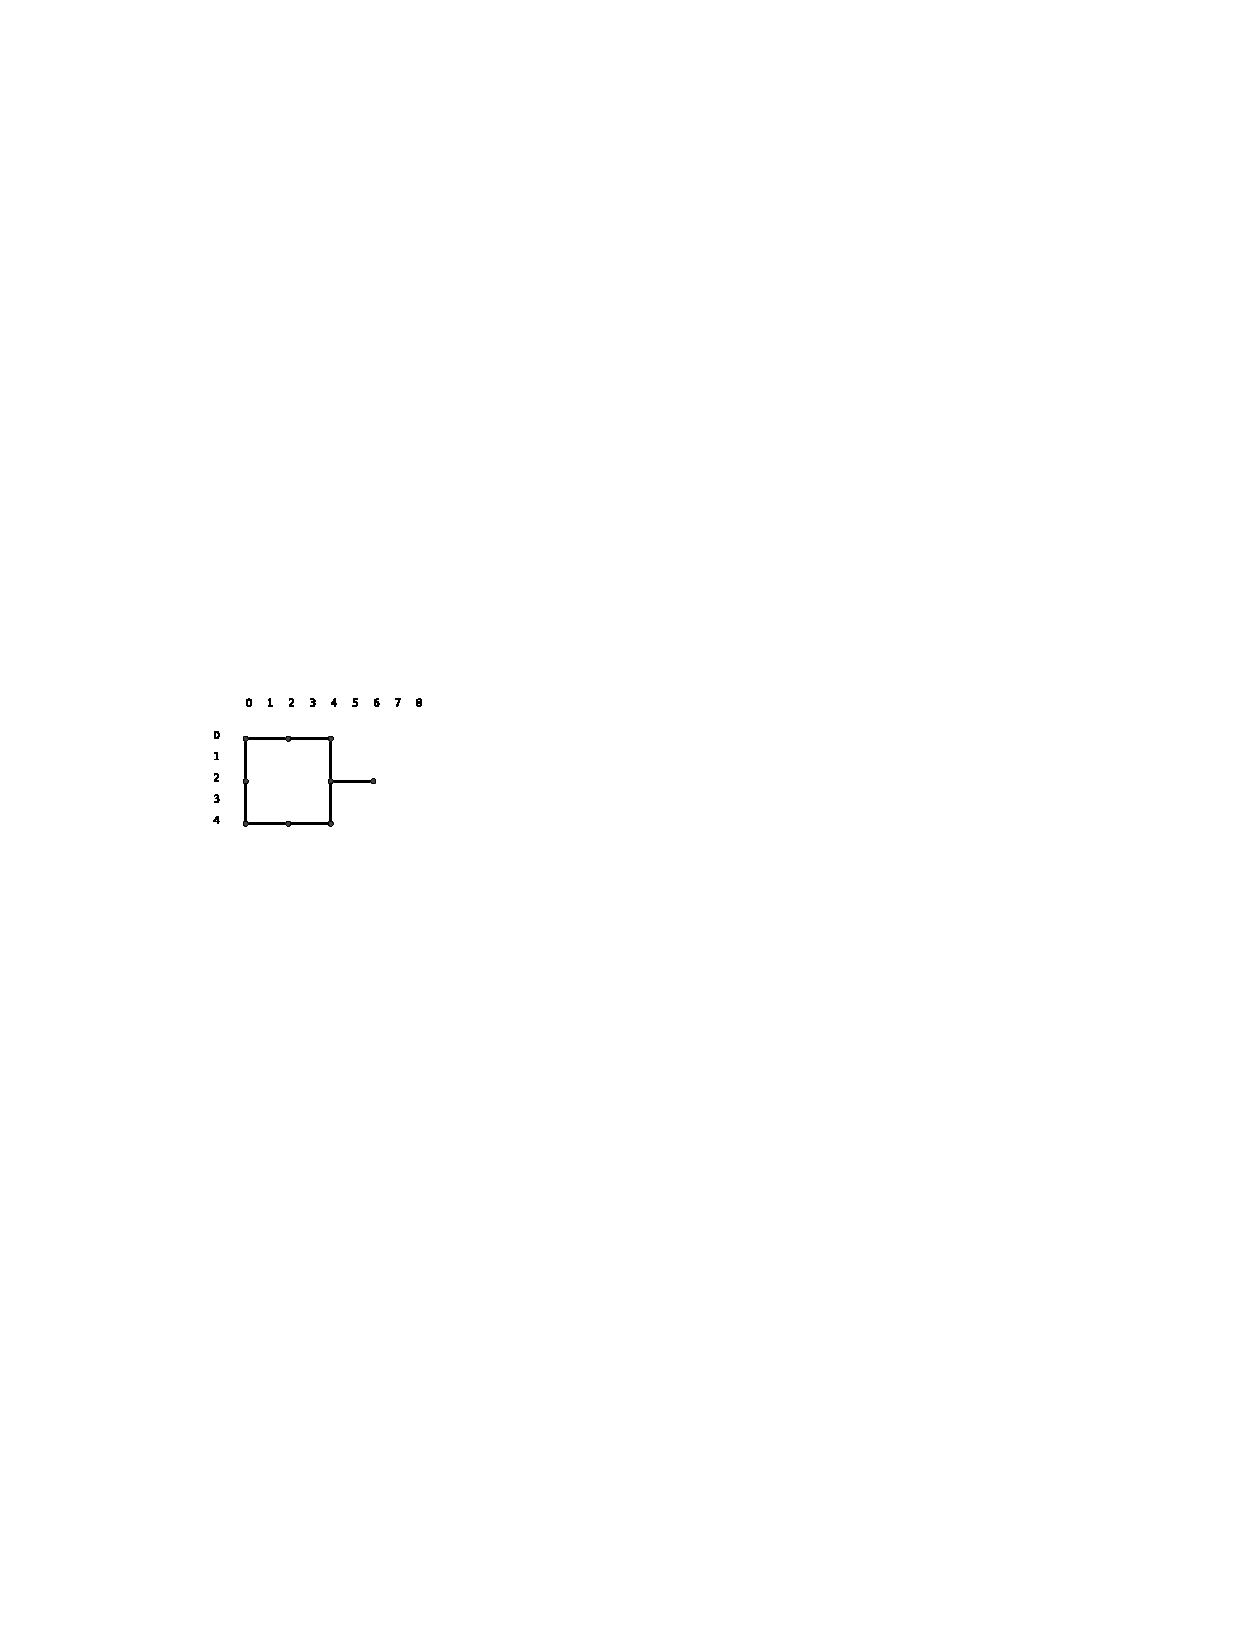
\includegraphics[trim=35mm 135mm 135mm 115mm, clip]{Example-09.pdf}}
\subfigure[]{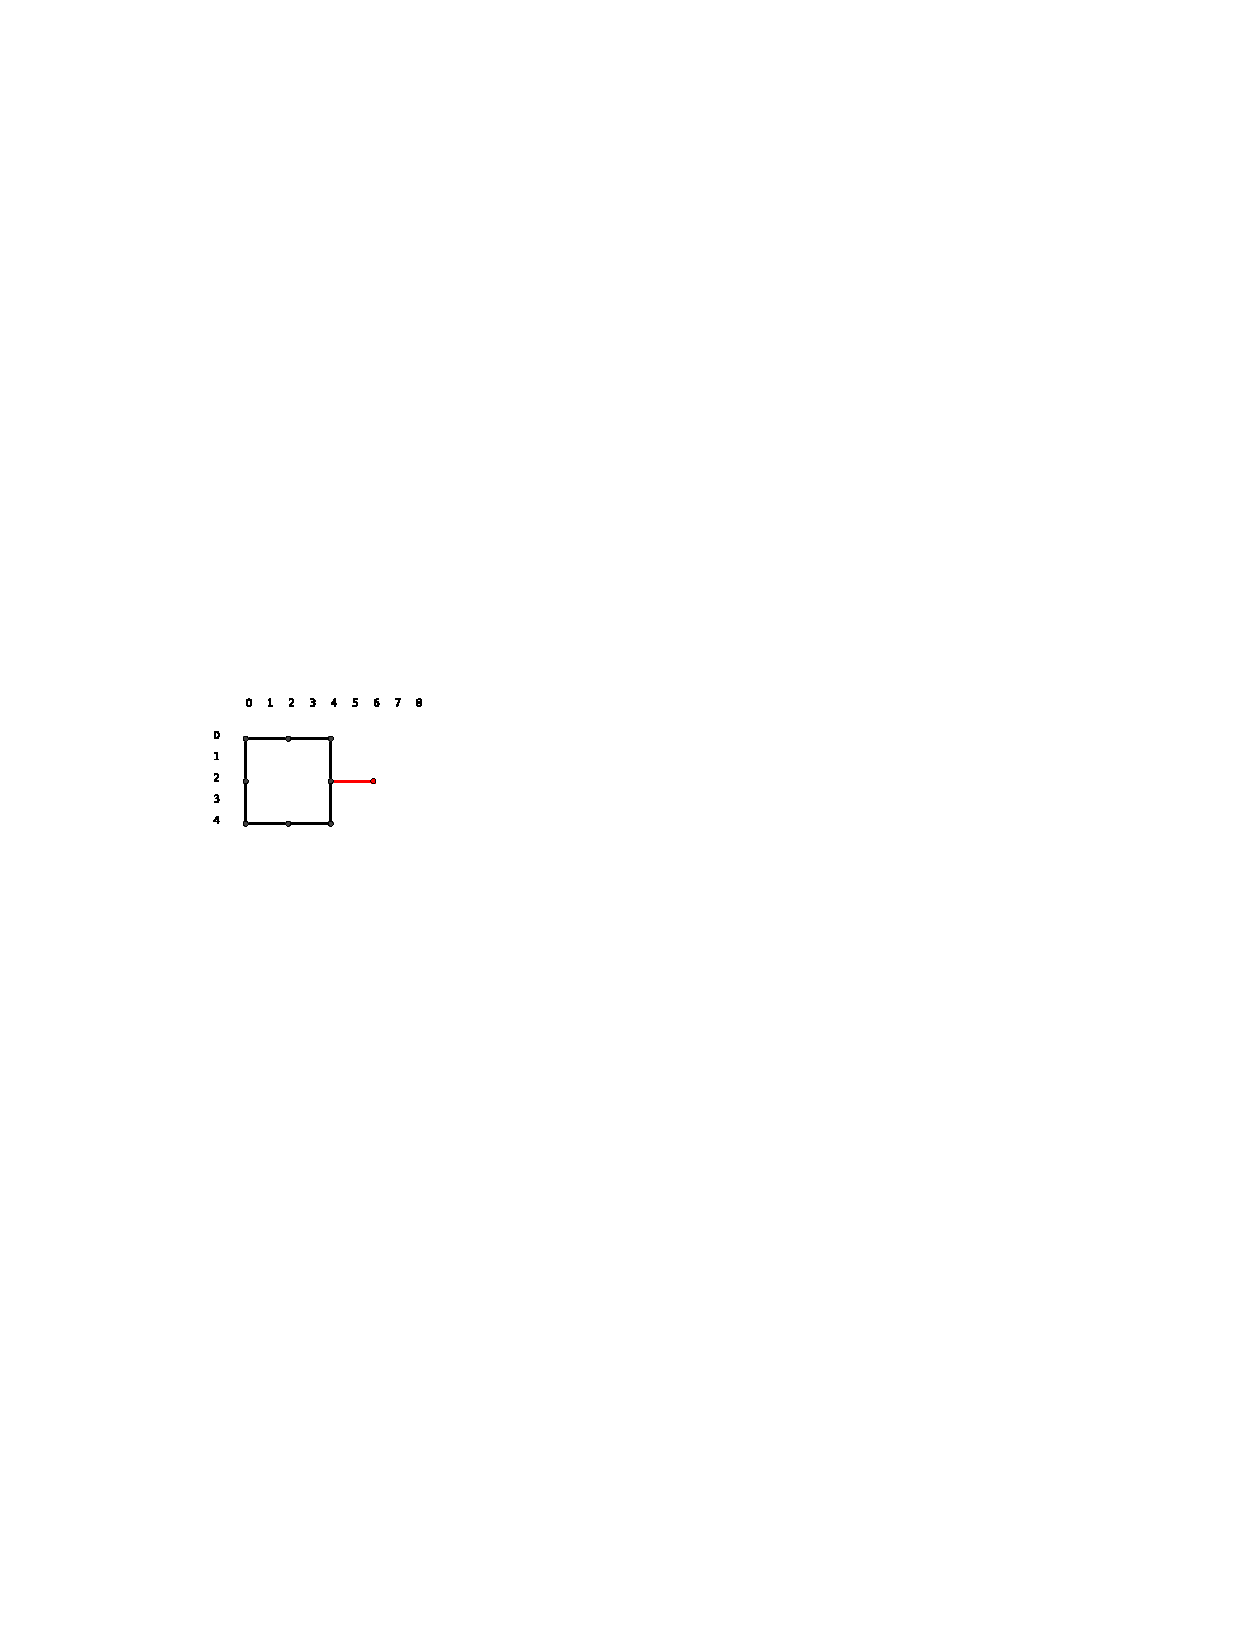
\includegraphics[trim=35mm 135mm 135mm 115mm, clip]{Example-10.pdf}}
\subfigure[]{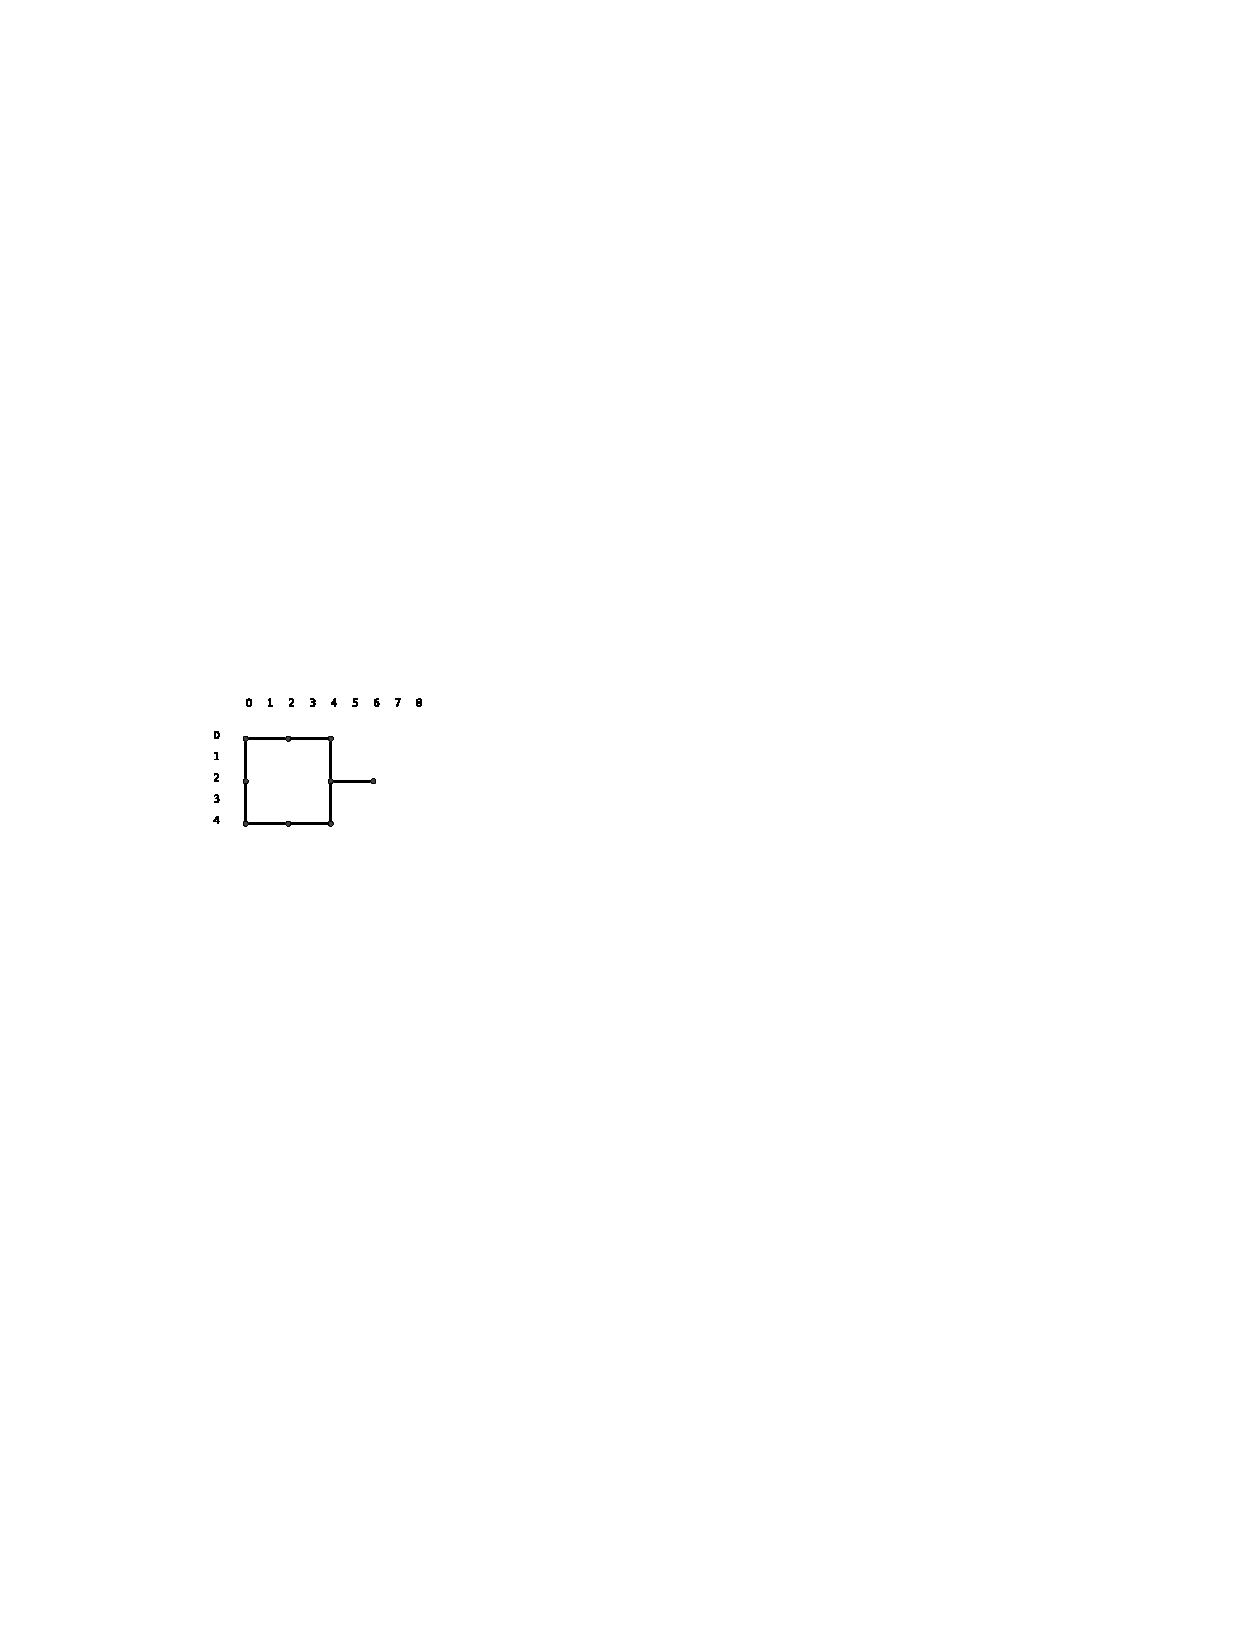
\includegraphics[trim=35mm 135mm 135mm 115mm, clip]{Example-09.pdf}}
\caption{Construction of a cubical complex associated to a binary image (a). In (b) the complex is shown over the image. In (c) the complex is shown alone. From (e) to (i) the thinning process is sketched.}
\end{figure}
\section{Conclusions and Future Work}
In this paper, three different research areas are brought together
in order to propose a new point of view on a classical problem:
Algebraic Topology, Membrane Computing and Digital Image Analysis.
Firstly, Algebraic Topology allows us to split the space in discrete
units and to define mechanical operators on such space units of
different dimensions. Secondly, a recent bio-inspired computational
model, Membrane Computing, is used to handle with such operators and
provide an alternative point of view for handling with them. Both
disciplines deal with compartments of the Euclidean space on their
foundations, but their inspiration and motivation are quite
different. The former is born as a tool for handle concepts of
Algebraic Topology and the latter is a computation model inspired in
the functioning of living cells and tissues.

The case of study for applying the Membrane Computing implementation of the
Algebraic Topology concepts has been the skeletonization problem, a classical
case study in Digital Image Analysis. This implementation provides a new proof
that the Membrane Computing framework is flexible enough to adapt to unexpected
situations. This paper follows the research line open with
\cite{ChristinalDR10}, but, to the best of our knowledge, this is the first work
which put together Membrane Computing, cells complexes and thinning processes.
In this way, this is a pioneer work that open a new research line that can be
followed at different levels.

Further research can be made by exploring other P system models with new
computational features, the application of Membrane Computing techniques to
further Digital Image Analysis or a deeper theoretical study of the
compartmental view of the Euclidean space by Membrane Computing and Algebraic
Topology as the starting point for a deeper study of their common properties.

\section*{Acknowledgements}
DDP and MAGN acknowledge the support of the Project of Excellence with
{\it Investigador de Reconocida Val\'{\i}a} of the Junta de
Andaluc\'{\i}a, grant P08-TIC-04200. MAGN also acknowledges the
support of the project TIN2012-37434 of the Ministerio de
Econom\'{\i}a y Competitividad of Spain. Both projects are cofinanced
by FEDER funds.

\bibliographystyle{IEEEtran}
\bibliography{Thinning_seville}
\end{document}
